\documentclass[output=collectionpaper]{langsci/langscibook}


\title{%
Gender typology and gender (in)stability in Hindu Kush Indo-Aryan languages
}%
\shorttitlerunninghead{Gender in Hindu Kush Indo-Aryan}

\author{%
Henrik Liljegren
\affiliation{Stockholm University}
}%

% \chapterDOI{} %will be filled in at production

\abstract{%
This paper investigates the phenomenon of gender as it appears in 25 Indo-Aryan languages (sometimes referred to as ``Dardic'') spoken in the Hindu Kush-Karakorum region \textendash{} the mountainous areas of northeastern Afghanistan, northern Pakistan and the disputed territory of Kashmir. Looking at each language in terms of the number of genders present, to what extent these are sex-based or non-sex-based, how gender relates to declensional differences, and what systems of assignment are applied, we arrive at a micro-typology of gender in Hindu Kush Indo-Aryan, including a characterization of these systems in terms of their general complexity. Considering the relatively close genealogical ties, the languages display a number of unexpected and significant differences. While the inherited sex-based gender system is clearly preserved in most of the languages, and perhaps even strengthened in some, it is curiously missing altogether in others (such as in Kalasha and Khowar) or seems to be subject to considerable erosion (e.g.\ in Dameli). That the languages of the latter kind are all found at the northwestern outskirts of the Indo-Aryan world suggests non-trivial interaction with neighbouring languages without gender or with markedly different assignment systems. In terms of complexity, the southwestern-most corner of the region stands out; here we find a few languages (primarily belonging to the Pashai group) that combine inherited sex-based gender differentiation with animacy-related distinctions resulting in highly complex agreement patterns. The findings are discussed in the light of earlier observations of linguistic areality or substratal influence in the region, involving Indo-Aryan, Iranian, Nuristani, Tibeto-Burman, Turkic languages and Burushaski. The present study draws from the analysis of earlier publications as well as from entirely novel field data.
\medskip

\textbf{Keywords:} Afghanistan, animacy, complexity, Dardic, gender pervasiveness, Indo-Aryan, Kashmir, non-sex-based gender, Pakistan, sex-based gender.
}%

\maketitle
\begin{document}
\label{ch:Liljegren}

\section{Introduction}
\label{sec:Lilje:1}

At the very northern fringe of the \ili{Indo-Aryan} world (approximately what lies north of the 34\textsuperscript{th} parallel) we find a group of languages that historically and culturally are somewhat outside the sphere of the main \ili{Indo-Aryan} languages of the subcontinent (\citealt[20--21]{Masica1991}). Geographically, this group is wedged in between \ili{Iranian} on its western side and \ili{Tibeto-Burman} on its eastern side, and the distance to the \ili{Turkic} belt of Central Asia is negligible at its farthest extension, even if it is not immediately adjacent.
This extremely mountainous and multilingual region (see \figref{fig:Lilje:1}), lies where the territories of Afghanistan, Pakistan and India-administered Kashmir meet. Henceforth, I will refer to this region as the Hindu Kush.%
\footnote{
Strictly speaking, this region only partly overlaps with the Hindu Kush mountain range, while also overlapping with the Karakorum and the westernmost extension of the Himalayas.
} %
Apart from the languages and genera already mentioned, this region is also home to \ili{Nuristani} \textendash{} a third, but numerically small, branch of \ili{Indo-Iranian} (\citealt[297--298]{Strand1973}) \textendash{} and to the isolate \ili{Burushaski}.

The languages in question have been subject to a great deal of debate as to whether they are truly \ili{Indo-Aryan}, constitute a genealogical unit of their own, or represent (perhaps along with the \ili{Nuristani} languages) a transitional group between \ili{Indo-Aryan} and \ili{Iranian}. A term frequently used collectively for these languages is ``\ili{Dardic}''. However, few modern linguists use this term as anything else than a convenient umbrella term for a group of languages that are characterized \textendash{} but not equally so \textendash{} by a few salient retentions from previous stages of \ili{Indo-Aryan} \citep[3]{Morgenstierne1974}, but also have some contact-related developments in common (\citealt[821--822]{Bashir2003}). Contact in that case includes mutual contact between the various \ili{Indo-Aryan} linguistic communities as well as significant contact with adjacent communities belonging to other genera \citep{Liljegren2017}. This non-committal line is also taken here regarding this grouping, but in order to avoid a stronger interpretation of ``\ili{Dardic}'' than warranted, the term is  abandoned in favour of \ili{Hindu Kush Indo-Aryan} (HKIA) (\citealt[135]{Liljegren2014}; \citealt[23]{HeegardPetersen2015}), again without any claim of classificatory significance in the traditional sense. While the region for quite some time has been identified as particularly interesting in terms of areality and language contact (\citealt{Emeneau1965}; \citealt{Skalmowski1985}; \citealt[43]{Masica1991}; \citealt[259]{Masica2001}), and a number of features have been suggested as characteristic (\citealt[392--420]{Bashir1988}; \citealt{Bashir1996}; \citealt[821--823]{Bashir2003}; \citealt{Edelman1980}; \citealt[35--59]{Edelman1983}; \citealt[389--399]{Fussman1972}; \citealt{Tikkanen1999,Tikkanen2008}; \citealt{Baart2014}; \citealt{Toporov1970}), relatively little detailed and systematic areal-linguistic research has been carried out so far.

\begin{figure}
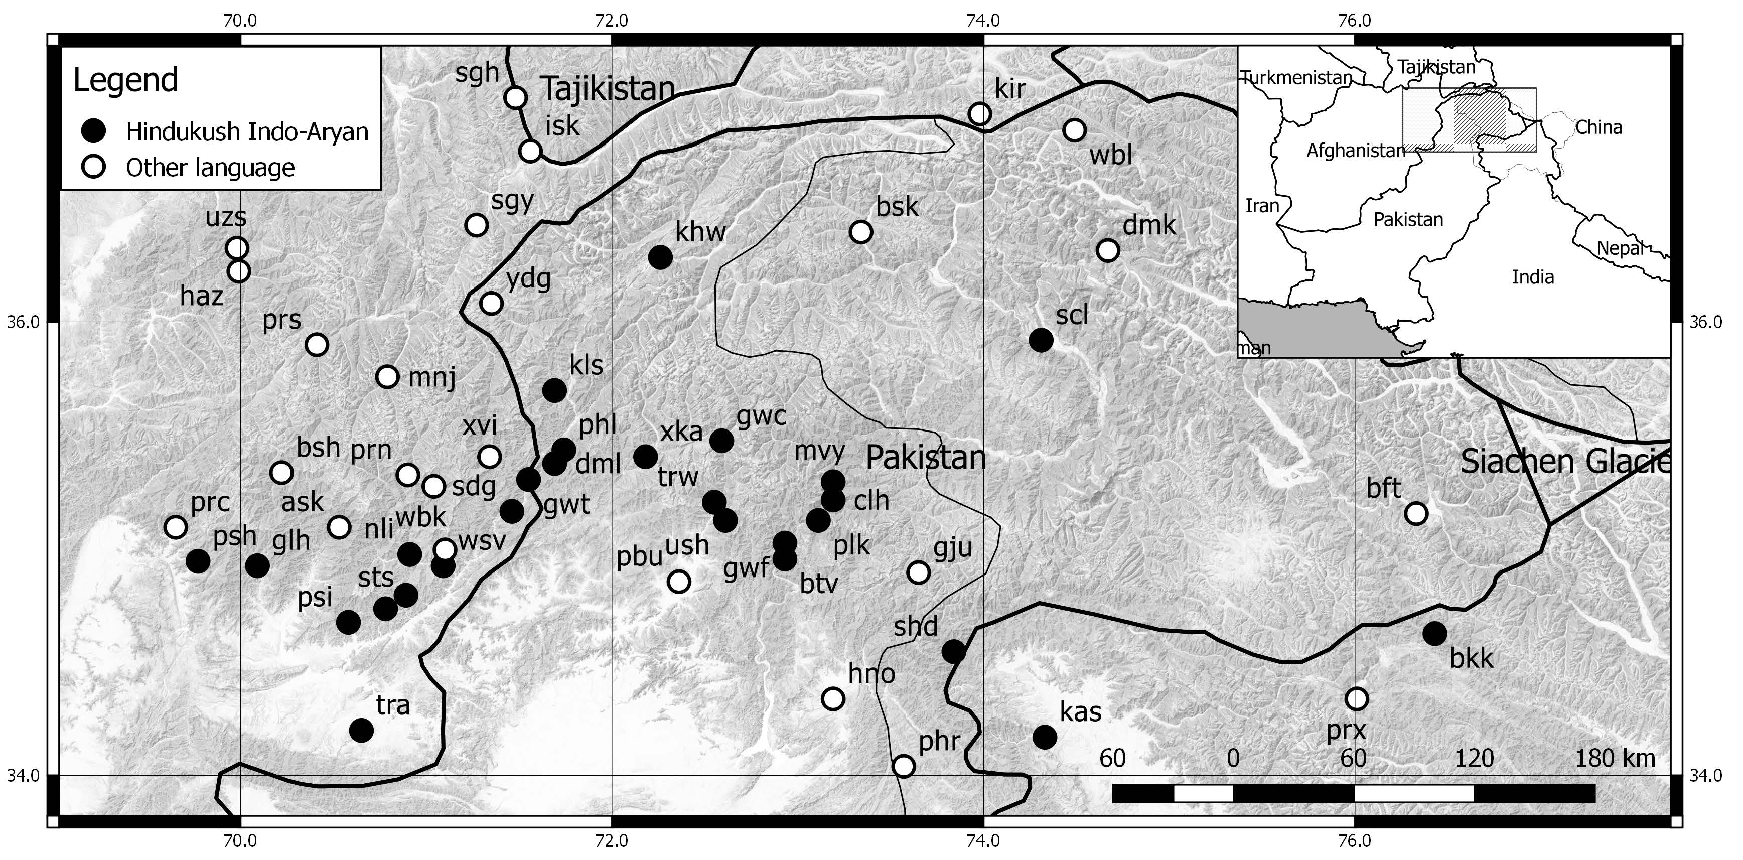
\includegraphics[width=\textwidth]{figures/10/map1}
\caption{The Hindu Kush-Karakoram region with languages plotted (see \tabref{tab:Lilje:1} for an explanation of the 3-letter codes)}
\label{fig:Lilje:1}
\end{figure}

Regarding the ancestral nominal system, evidenced in Old \ili{Indo-Aryan} as well as in Middle \ili{Indo-Aryan}, it encompassed three gender values: masculine, feminine and neuter. In the \ili{Indo-Aryan} world in general, these three values are only preserved in the modern languages in the southern part of the subcontinent, whereas a simplified two-value system (masculine vs.\ feminine, mainly as a result of neuter collapsing with masculine) dominates the large central and western parts. Such distinctions have altogether vanished in the northeast (\citealt[217--223]{Masica1991}). The somewhat unexpected distribution and display of grammatical gender in the languages at the northern and western frontier of \ili{Indo-Aryan} (viz.\ the Hindu Kush) was pointed out by \citet[68--71]{Emeneau1965} half a century ago, but apart from Morgenstierne's (\citeyear[19--20]{Morgenstierne1950}) tabulation, no systematic attempt has to my knowledge been made to account for gender distribution and manifestation across HKIA. This study tries to rectify that by showing the results of a survey of the following gender-related features \textendash{} partly inspired by a number of contributions to the \textit{World atlas of language structures} (\textit{WALS}) \textendash{} for each HKIA language for which there is data:

\begin{itemize}
\item
The presence and number of gender categories (as evidenced by agreement patterns), and their basis, whether sex-based or non-sex-based (\citealt{Corbett2013,Corbett2013a}).
\item
The pervasiveness of gender, i.e.\ how gender is manifested in each language system in terms of (the types and numbers of) indexed domains.
\item
The assignment criteria at work: whether semantic or semantic-formal \citep{Corbett2013b}.
\item
The presence and manifestation of pronominal gender \citep{Siewierska2013}.
\end{itemize}

In the process of discussing and summarising these results, particularly in terms of the relative complexity of these systems, and in the light of areal patterning, a micro-typology of gender in HKIA emerges:

\begin{itemize}
\item
The inherited sex-based system is largely preserved, but has disappeared in two of the languages at the Northwestern fringe of the Hindu Kush and is possibly eroding in a few other languages spoken in the same part of the region.
\item
An animacy-based system (almost exclusively marked on copulas or copula-based verbal categories) characterizes a number of the western-most languages of the region. In some cases it co-exists with a sex-based system; in others it occurs instead of a sex-based system or has contributed to a restructuring of the system as a whole.
\item
Gender is deeply entrenched (reflected in more target domains) in the East, i.e.\ in the languages spoken in areas contiguous with the main \ili{Indo-Aryan} belt, whereas such pervasiveness is fading out toward the West.
\item
The results also suggest a weaker tendency toward semantic transparency in the gender systems in the North and a reinforcement of formal assignment, along with object agreement, in the South.
\end{itemize}


\section{Hindu Kush Indo-Aryan and other languages in the region}

Today, there are 28 distinct HKIA languages,\il{Hindu Kush Indo-Aryan} i.e.\ languages identified as ``\ili{Dardic}'' by the language catalogue Ethnologue (\citealt{Eberhard2019}), spoken in the region, the great majority of them on Pakistani soil or in areas of Kashmir now under Pakistani control. At least six clusters of related languages can be identified, mainly going with Bashir (\citeyear[824--825]{Bashir2003}) and the classification used in Glottolog (\citealt{Hammarstroem2018}), although the definitive placement of a few of the individual languages is still pending (\ili{Dameli}, \ili{Tirahi} and \ili{Wotapuri-Katarqalai}). All HKIA languages\il{Hindu Kush Indo-Aryan} are presented in \tabref{tab:Lilje:1}, roughly according to their geographical distribution, from west to east in a crescent-like fashion (see \figref{fig:Lilje:1}). No attempt has been made here to represent relatedness below the level of these six groupings.


\begin{table}[p]
\small
\begin{tabularx}{\textwidth}{lll>{\raggedright\let\newline\\\arraybackslash\hspace{0pt}}X}
\lsptoprule
Group & Language & code & Area (Country)\\
\midrule
\ili{Pashai} & Northwest Pashai\il{Pashai, Northwest} & [glh] & Kabul, Kapisa, Konar, Laghman, Nurestan (Afg)\\
& Southwest Pashai\il{Pashai, Southwest} & [psh] & Kabul, Kapisa (Afg)\\
& Southeast Pashai\il{Pashai, Southeast} & [psi] & Nangarhar, Laghman (Afg)\\
& Northeast Pashai\il{Pashai, Northeast} & [aee] & Konar, Nangarhar (Afg)\\
\ili{Kunar} & \ili{Shumashti} & [sts] & Konar (Afg)\\
& \ili{Grangali} & [nli] & Konar, Nangarhar (Afg)\\
& \ili{Gawarbati} & [gwt] & Konar (Afg), \ili{Chitral} (Pak)\\
& \ili{Dameli} & [dml] & \ili{Chitral} (Pak)\\
\ili{Chitral} & \ili{Kalasha} & [kls] & \ili{Chitral} (Pak)\\
& \ili{Khowar} & [khw] & \ili{Chitral}, Gilgit-Baltistan (Pak)\\
\ili{Kohistani} & \ili{Tirahi} & [tra] & Nangarhar (Afg)\\
& \ili{Wotapuri-Katarqalai} & [wsv] & Nurestan (Afg)\\
& \ili{Gawri} (\ili{Kalami}) & [gwc] & Upper Dir, Swat (Pak)\\
& \ili{Torwali} & [trw] & Swat (Pak)\\
& Indus Kohistani\il{Kohistani, Indus} & [mvy] & Kohistan (Pak)\\
& \ili{Gowro} & [gwf] & Kohistan (Pak)\\
& \ili{Chilisso} & [clh] & Kohistan (Pak)\\
& \ili{Bateri} & [btv] & Kohistan (Pak)\\
& \ili{Mankiyali} & [nlm] & Mansehra (Pak)\\
\ili{Shina} & \ili{Sawi} & [sdg] & Konar (Afg)\\
& \ili{Palula} & [phl] & \ili{Chitral} (Pak)\\
& \ili{Kalkoti} & [xka] & Upper Dir (Pak)\\
& \ili{Ushojo} & [ush] & Swat (Pak)\\
& \ili{Kohistani} \ili{Shina} & [plk] & Kohistan (Pak)\\
& \ili{Kundal Shahi} & [shd] & Jammu \& Kashmir (Pak)\\
& Shina (Gilgiti)\il{Shina, Gilgiti} & [scl] & Gilgit-Baltistan (Pak), Jammu \& Kashmir (Ind)\\
& \ili{Brokskat} & [bkk] & Jammu \& Kashmir (Ind)\\
\ili{Kashmiri} & Standard \ili{Kashmiri} & [kas] & Jammu \& Kashmir (Ind), Jammu \& Kashmir (Pak)\\
\lspbottomrule
\end{tabularx}
\caption{Hindu Kush Indo-Aryan languages (with 3-letter ISO codes and the areas and countries where they are spoken), arranged in sub-groupings}
\label{tab:Lilje:1}
\end{table}


Some of these groupings are tighter, i.e.\ internally less diverse, than others. This is one reason why they sometimes are treated as single languages with a number of dialects rather than as groupings of separate languages. That especially applies to \ili{Kashmiri}, \ili{Shina} and \ili{Pashai}. The relatedness between the two \ili{Chitral} group languages, \ili{Khowar} and \ili{Kalasha}, is also apparent from a number of features that single these two out from the rest of HKIA. The latter two were assumed by \citet[51]{Morgenstierne1932} to represent the first wave of \ili{Indo-Aryan} settlers moving in from the lowlands in the South.

If we, for the sake of simplicity, define the Hindu Kush region as the window between the longitudes 34 and 37 N and the latitudes 69 and 77 E, another 25 languages are spoken here. At least four other languages (or continua), traditionally described as belonging to sub-branches of \ili{Indo-Aryan} with their geographical centres outside of the Hindu Kush region, are also found in the Hindu Kush region, or their geographical extension overlaps to a considerable extent with it: \ili{Hindko} [hno], \ili{Pahari-Pothwari} [phr], \ili{Gojri} [gju] and \ili{Domaaki} [dmk]. \ili{Hindko} and \ili{Pahari-Pothwari} are essentially part of a \ili{Punjabi} macro-language extended far beyond the region, and as such they represent the closest main \ili{Indo-Aryan} neighbour of HKIA. \ili{Gojri} is the language of nomadic or semi-nomadic Gujurs, spoken in pockets throughout the region and beyond. The closest linguistic relatives of Rajasthani \ili{Indo-Aryan} \ili{Gojri} is, however, to be found at a considerable distance from the present region, deep into the main belt of \ili{Indo-Aryan}. The closest relatives of \ili{Domaaki} are likewise to be found in the plains of North India. \ili{Domaaki}, however, is interesting from an areal point of view; as the language of a small enclave of  musicians and blacksmiths surrounded by locally dominant speaker groups of \ili{Shina} and \ili{Burushaski}, it has during its 200--300 years in the area acquired a number of features typical of HKIA (\citealt[165--166]{Weinreich2011}).

A number of the surrounding languages in the West are \ili{Iranian}. \ili{Pashto} [pbu] and \ili{Dari} [prs], the two representing two completely different branches of \ili{Iranian}, are both important lingua francas in parts of the region and well beyond. \ili{Dari} is essentially the standard or literary type of Eastern \ili{Persian} used in Afghanistan, while various names occur in reference to regional or local varieties, such as \ili{Tajik} in north-eastern Afghanistan and neighbouring Tajikistan. Some of those may very well be considered languages in their own rights, e.g.\ \ili{Hazaragi} [haz]. Most of the other \ili{Iranian} languages (all very distantly related to either \ili{Pashto} or \ili{Dari}) are relatively minor, with a local scope only; in Afghanistan, \ili{Parachi} [prc], \ili{Munji} [mnj], \ili{Sanglechi} [sgy], \ili{Ishkashimi} [isk] and \ili{Shughni} [sgh]; in Pakistan, \ili{Yidgha} [ydg], basically a dialect of the same language as \ili{Munji}; in Pakistan and Afghanistan as well as in adjacent areas of Tajikistan and China, \ili{Wakhi} [wbl] is spoken.

All of the five to six \ili{Nuristani} languages are spoken in a geographically confined area in Afghanistan's Nurestan Province, close to the Pakistan border (with some spill-over into adjacent \ili{Chitral}): \ili{Kati} [bsh], \ili{Kamviri} [xvi] (more correctly a dialect rather than a separate language from the aforementioned), \ili{Waigali} [wbk], \ili{Ashkun} [ask], \ili{Tregami} [trm] and \ili{Prasun} [prn]. Two \ili{Turkic} languages are spoken at the northern periphery of the region: \ili{Uzbek} [uzs] and \ili{Kirghiz} [kir]; and in the East two with each other closely related \ili{Tibeto-Burman} languages are found: \ili{Balti} [bft] and \ili{Purik} [prx]. The already-mentioned language isolate \ili{Burushaski} is spoken in the extreme North of Pakistan's Gilgit-Baltistan region.

\section{Sample and data}
The sparsity of data points in large-scale typological enterprises such as \textit{WALS} stresses the need for different selectional criteria when it comes to areal\hyp{}typological or micro-typological studies. For instance, three of the \textit{WALS} features (30A, 31A, 32A) that deal with gender include in their 257-language sample only five of the languages spoken in the Hindu Kush (\ili{Burushaski}, \ili{Kashmiri}, \ili{Kirghiz}, \ili{Pashto} and \ili{Uzbek}), and of them only one (\ili{Kashmiri}) is a HKIA language (\citealt{Corbett2013,Corbett2013a,Corbett2013b}). For the feature surveying pronominal gender (44A), the corresponding figures are 2 (\ili{Burushaski} and \ili{Kashmiri}) and 1 (\ili{Kashmiri}), respectively, in a world-wide 378-language sample \citep{Siewierska2013}.

It was therefore the aim of this survey to draw data from as many as possible of the 28 above-mentioned HKIA languages,\il{Hindu Kush Indo-Aryan} rather than trying to identify and justify a smaller sample. This posed some challenges, as the quality and amount of documentation vary greatly from language to language. However, by combining available published descriptions with my own field data from a variety of languages in the region, it has been possible to find out which are the main characteristics and values (as presented in \sectref{sec:Lilje:1}) for as many as 25 of them. I saw a definite need to exclude \ili{Gowro}, \ili{Chilisso} and \ili{Mankiyali} due to lack of adequate data, but this should probably not distort the overall picture in any significant way, since the preliminary analysis shows that at least Gowro and Chilisso are relatively closely linked to Indus Kohistani\il{Kohistani, Indus} \citep[874]{Bashir2003}. The addition of unpublished field data was particularly important concerning the under-researched languages \ili{Bateri}, \ili{Kalkoti} and \ili{Ushojo}. In \tabref{tab:Lilje:2}, the sources of information for each language are specified.

%
%\begin{table}[p]
%\small
%\begin{tabularx}{\textwidth}{l>{\raggedright\let\newline\\\arraybackslash\hspace{0pt}}Xl>{\raggedright\let\newline\\\arraybackslash\hspace{0pt}}X}
%\lsptoprule
%
%Language & Sources & Language & Sources\\
%\midrule
%\ili{Northwest Pashai} & (\citealt[143--203]{Morgenstierne1967}); own data & \ili{Torwali} & (\citealt{Lunsford2001}; \citealt[864--869]{Bashir2003}; \citealt{Grierson1929}); own data\\
%Southwest \ili{Pashai} & (\citealt[45--142]{Morgenstierne1967}) & Indus Kohistani & (\citealt{Hallberg1999}; \citealt[874--877]{Bashir2003}; \citealt{Lubberger2014}); own data\\
%Southeast \ili{Pashai} & (\citealt[251--297]{Morgenstierne1967}; \citealt{Lehr2014}); own data & \ili{Bateri} & (\citealt[207--225, 249--251]{Hallberg1992}); own data\\
%\ili{Northeast Pashai} & (\citealt[205--249]{Morgenstierne1967}); own data & \ili{Sawi} & (\citealt{Buddruss1967}; \citealt[43--48]{Liljegren2009}); own data\\
%\ili{Shumashti} & \citep{Morgenstierne1945} & \ili{Palula} & \citep{Liljegren2016}; own data\\
%\ili{Grangali} & (\citealt[837--839]{Bashir2003}; \citealt{Grjunberg1971}) & \ili{Kalkoti} & (\citealt[43--48]{Liljegren2009}; \citealt{Liljegren2013}); own data\\
%\ili{Gawarbati} & \citep{Morgenstierne1950}; own data & \ili{Ushojo} & \citep{Decker1992}; own data\\
%\ili{Dameli} & (\citealt{Morgenstierne1942}; \citealt{Perder2013}); own data & \ili{Kohistani} \ili{Shina} & (\citealt{Schmidt2008}); own data\\
%\ili{Kalasha} & (\citealt[35--49]{HeegardPetersen2015}; \citealt{Bashir1988}); own data & \ili{Kundal Shahi} & ( \citealt{Rehman2005}); own data\\
%\ili{Khowar} & (\citealt[844--849]{Bashir2003}); own data & \ili{Shina} (\ili{Gilgiti}) & (\citealt{Bailey1924}; \citealt[13--65]{Degener2008}; \citealt[183--192]{Radloff1998}); own data\\
%\ili{Tirahi} & (\citealt{Morgenstierne1934a}; \citealt[265--327]{Grierson1927}) & \ili{Brokskat} & (\citealt{Ramaswami1982}; \citealt{Sharma1998})\\
%\ili{Wotapuri-Katarqalai} & \citep{Buddruss1960} & Standard \ili{Kashmiri} & (\citealt{Koul2003}; \citealt[175--211]{Verbeke2013}); own data\\
%\ili{Gawri} (\ili{Kalami}) & (\citealt{Baart1997,Baart1999}); own data &  & \\
%\lspbottomrule
%\end{tabularx}
%\caption{Data sources for Hindu Kush Indo-Aryan}
%\label{tab:Lilje:2}
%\end{table}


%%%%%%%%%%%%%%%%%%%%%%%%%%%%%%%%%%%%
%%%%%%%%% ALTERNATIVE TABLE BY BRUNO %%%%%%%%%
%%%%%%%%%%%%%%%%%%%%%%%%%%%%%%%%%%%%

\begin{table}[p]
%\small
\begin{tabularx}{\textwidth}{l>{\raggedright\let\newline\\\arraybackslash\hspace{0pt}}X}
\lsptoprule

Language & Sources \\
\midrule
Northwest Pashai\il{Pashai, Northwest} & (\citealt[143--203]{Morgenstierne1967}); own data \\
Southwest Pashai\il{Pashai, Southwest} & (\citealt[45--142]{Morgenstierne1967}) \\
Southeast Pashai\il{Pashai, Southeast} & (\citealt[251--297]{Morgenstierne1967}; \citealt{Lehr2014}); own data \\
Northeast Pashai\il{Pashai, Northeast} & (\citealt[205--249]{Morgenstierne1967}); own data \\
\ili{Shumashti} & \citep{Morgenstierne1945} \\
\ili{Grangali} & (\citealt[837--839]{Bashir2003}; \citealt{Grjunberg1971}) \\
\ili{Gawarbati} & \citep{Morgenstierne1950}; own data \\
\ili{Dameli} & (\citealt{Morgenstierne1942}; \citealt{Perder2013}); own data \\
\ili{Kalasha} & (\citealt[35--49]{HeegardPetersen2015}; \citealt{Bashir1988}); own data \\
\ili{Khowar} & (\citealt[844--849]{Bashir2003}); own data \\
\ili{Tirahi} & (\citealt{Morgenstierne1934a}; \citealt[265--327]{Grierson1927}) \\
\ili{Wotapuri-Katarqalai} & \citep{Buddruss1960} \\
\ili{Gawri} (\ili{Kalami}) & (\citealt{Baart1997,Baart1999}); own data \\
\ili{Torwali} & (\citealt{Lunsford2001}; \citealt[864--869]{Bashir2003}; \citealt{Grierson1929}); own data \\
Indus Kohistani\il{Kohistani, Indus} & (\citealt{Hallberg1999}; \citealt[874--877]{Bashir2003}; \citealt{Lubberger2014}); own data \\
\ili{Bateri} & (\citealt[207--225, 249--251]{Hallberg1992}); own data \\
\ili{Sawi} & (\citealt{Buddruss1967}; \citealt[43--48]{Liljegren2009}); own data \\
\ili{Palula} & \citep{Liljegren2016}; own data \\
\ili{Kalkoti} & (\citealt[43--48]{Liljegren2009}; \citealt{Liljegren2013}); own data \\
\ili{Ushojo} & \citep{Decker1992}; own data \\
\ili{Kohistani} \ili{Shina} & (\citealt{Schmidt2008}); own data \\
\ili{Kundal Shahi} & (\citealt{Rehman2005}); own data \\
Shina (Gilgiti)\il{Shina, Gilgiti} & (\citealt{Bailey1924}; \citealt[13--65]{Degener2008}; \citealt[183--192]{Radloff1998}); own data \\
\ili{Brokskat} & (\citealt{Ramaswami1982}; \citealt{Sharma1998}) \\
Standard \ili{Kashmiri} & (\citealt{Koul2003}; \citealt[175--211]{Verbeke2013}); own data \\
\lspbottomrule
\end{tabularx}
\caption{Data sources for Hindu Kush Indo-Aryan}
\label{tab:Lilje:2}
\end{table}

%%%%%%%%%%%%%%%%%%%

\section{Gender Categories and their basis}
\label{sec:Lilje:4}
The first question to address is whether gender a distinctive feature; and, if it is, also how many genders there are in the language. Here I align myself with the view that membership in a particular gender category in contrast with one or more other such categories in the language in question is inherent to a noun but has to be evidenced by grammatical contrasts outside the noun itself, for instance in the form of adjectival or verbal agreement (\citealt[89--90]{Corbett2014}; \citealt[231--233]{Hockett1958}; \citealt[50]{Greenberg1978}). Another relevant question is whether the gender system is based on, or primarily linked to, biological sex, or to something other than sex. Surveying the languages in our sample, we find (\tabref{tab:Lilje:3}) that all of them display gender
distinctions, one way or the other, with the possible exception of some dialects of NW \ili{Pashai}.
%
\footnote{%
The preliminary analysis of my own data, from three NW \ili{Pashai} locations (Sanjan, Alasai and Alishang) indicates the overall presence of sex-based adjectival gender agreement, whereas clear evidence of animacy-based differentiation is lacking in these particular varieties. While those findings have guided the present treatment, Morgenstierne's (\citeyear[150--151, 173--176]{Morgenstierne1967}) study suggests a great deal of dialectal variation within NW \ili{Pashai} as far as the presence/absence of both sex-based and animacy-based gender are concerned.} %


\begin{table}

\begin{tabularx}{\textwidth}{lXXX}
\lsptoprule
Language & Number of genders & Sex-based gender & Non-sex-based gender\\
\midrule
Southwest Pashai\il{Pashai, Southwest} & 4 & \cmark  & \cmark \\
Southeast Pashai\il{Pashai, Southeast} & 4 & \cmark  & \cmark \\
Northeast Pashai\il{Pashai, Northeast} & 4 & \cmark  & \cmark \\
\ili{Shumashti} & 3--4 & \cmark  & \cmark \\
\ili{Dameli} & 3 & \cmark  & \cmark \\
\ili{Kalasha} & 2 &  & \cmark \\
\ili{Khowar} & 2 &  & \cmark \\
Northwest Pashai\il{Pashai, Northwest} & 2 & \cmark  & \\
\ili{Grangali} & 2 & \cmark  & \\
\ili{Gawarbati} & 2 & \cmark  & \\
\ili{Tirahi} & 2 & \cmark  & \\
\ili{Wotapuri-Katarqalai} & 2 & \cmark  & \\
\ili{Gawri} (\ili{Kalami}) & 2 & \cmark  & \\
\ili{Torwali} & 2 & \cmark  & \\
Indus Kohistani\il{Kohistani, Indus} & 2 & \cmark  & \\
\ili{Bateri} & 2 & \cmark  & \\
\ili{Sawi} & 2 & \cmark  & \\
\ili{Palula} & 2 & \cmark  & \\
\ili{Kalkoti} & 2 & \cmark  & \\
\ili{Ushojo} & 2 & \cmark  & \\
\ili{Kohistani} \ili{Shina} & 2 & \cmark  & \\
\ili{Kundal Shahi} & 2 & \cmark  & \\
Shina (Gilgiti)\il{Shina, Gilgiti} & 2 & \cmark  & \\
\ili{Brokskat} & 2 & \cmark  & \\
Standard \ili{Kashmiri} & 2 & \cmark  & \\
\lspbottomrule
\end{tabularx}
\caption{The presence of gender (sex-based, non-sex-based) in Hindu Kush Indo-Aryan}
\label{tab:Lilje:3}
\end{table}

As can also be seen in \tabref{tab:Lilje:3}, the basis for such distinctions is not the same for all of the languages. In the great majority of the languages (23 out of 25), the gender system, as it is mirrored in agreement, is clearly sex-based, having (at least) a two-way, female vs.\ male, differentiation at its core (as in many other \ili{Indo-Aryan} languages in general). This is seen in example (\ref{ex:Lilje:1}) from \ili{Ushojo}, where `boy' in (a) triggers masculine verb agreement, and `girl' in (b) triggers feminine agreement. This masculine--feminine differentiation also extends into the inanimate realm: `wind', in (c), is assigned feminine gender, and `coldness', in (d), is assigned masculine gender.

\protectedex{%
\ea
\label{ex:Lilje:1}
\langinfo{Ushojo}{}{Own data}\\
\begin{xlist}
\ex
\gll ek \textbf{phoó} asíl-\textbf{u}, se seekel-aá yáa áal-\textbf{u}.\\
one boy(\textsc{m}) be.\textsc{pst-m.sg} \textsc{3sg.nom} bicycle-\textsc{loc} going come.\textsc{pfv-m.sg}\\
\glt  `There was a boy, he came riding on a bicycle.' (USH-PearStoryAH:001)\\
\ex
\gll ek \textbf{phuí} ... seekal-aá yáa mušíin tarapayá áal-\textbf{i}.\\
one girl(\textsc{f}) {} bicycle-\textsc{loc} going to.near in.direction come.\textsc{pfv-f.sg}\\
\glt `A girl… came in his direction, riding on a bicycle.' (USH-PearStoryAH:012)\\
\ex
\gll axeér \textbf{oóš} čóku bíl-\textbf{i}.    \\
finally wind(\textsc{f}) quiet become.\textsc{pfv-f.sg}    \\
\glt `Finally the wind gave up.' (USH-NorthwindAH:007)
\ex
\gll maáti \textbf{šídal} bíl-\textbf{u}.     \\
\textsc{1sg.dat} coldness(\textsc{m}) become.\textsc{pfv-m.sg}     \\
\glt `I feel cold [lit.\ Coldness came to me].' (USH-ValQuestAH:060)
\end{xlist}
\z
}%

In two of the languages, \ili{Khowar} and \ili{Kalasha}, both belonging to the \ili{Chitral} group, sex-based differentiation is entirely lacking. However, in both languages we find a two-way differentiation based on animacy, where animate nouns (including humans and higher non-human animals) are treated differently from inanimate nouns by some agreement targets. For instance, the present actual copula verb used in locational predication in \ili{Khowar} has different third person singular and plural agreement forms for animate and inanimate, respectively. That is illustrated in example (\ref{ex:Lilje:2}) with the two plural forms. (The corresponding singular forms are \textbf{\textit{asú}}\textbf{\textit{r}} and \textbf{\textit{šer}}.) The copula, in its various forms, is also used as an auxiliary participating in some tense-aspect formations.

\ea
\label{ex:Lilje:2}
\langinfo{Khowar}{}{Own data}\\
\begin{xlist}
\ex
\gll dúr-a \textbf{roy}  \textbf{asúni}.     \\
house-\textsc{loc} people(\textsc{an}) be\textsc{.prs.act.3.an.}\textsc{pl}     \\
\glt `There are people in the house.' (KHW-PredFA:011)\\
\ex
\gll \textbf{kitáb}  ma dúr-a  \textbf{šéni}.    \\
book(\textsc{inan}) \textsc{1sg.gen} house-\textsc{loc} be\textsc{.prs.act.3.inan.pl}    \\
\glt `The books are in my house.' (KHW-PredFA:009)\\
\end{xlist}
\z

A few of the dialects of NW \ili{Pashai} may also lack sex-based gender distinctions (\citealt[150--151]{Morgenstierne1967}); in those cases we do not have conclusive information on the presence of animacy distinctions. In another few languages \textendash{} in \ili{Dameli} and \ili{Shumashti} (both \ili{Kunar} languages), and in several of the \ili{Pashai} varieties \textendash{} animacy differentiation occurs, not instead of but in addition to sex-based differentiation. However, there are reasons to regard these as two separate features (with two values each) that affect different parts (or sub-domains) of the language system, a situation that \citet[581--582]{Dahl2000} refers to as ``parallel combinations of gender distinctions''. The feminine--masculine and animate--inanimate distinctions only marginally make use of the same agreement target. In \ili{Dameli}, this happens in non-verbal predication, which results in a three-way differentiation at the most: animate masculine vs.\ animate feminine vs.\ inanimate, as shown in example (\ref{ex:Lilje:3}). Apart from the specific domain of non-verbal predication in \ili{Dameli}, a two-way masculine vs.\ feminine distinction is upheld in most other parts of the grammar. It is not unlikely that a similar situation holds in \ili{Shumashti}, although the data available is too scanty to draw any firm conclusions.

\ea
\label{ex:Lilje:3}
\langinfo{Dameli}{}{Own data}\\*
\begin{xlist}
\ex
\gll i \textbf{mač} mruy \textbf{thaa}.    \\
\textsc{prox.an} man(\textsc{m}) hunter be\textsc{.prs.3m.sg}    \\
\glt `This man is a hunter.' (DML-ValQuestHM:070)\\
\ex
\gll \textbf{poši} koki \textbf{thui}.     \\
cat(\textsc{f}) asleep be.\textsc{prs.3f.sg}     \\
\glt `The cat is asleep.' (DML-ErgSurvHM:013)\\
\ex
\gll \textbf{bum} šukisan \textbf{daru}.     \\
ground dry be.\textsc{prs.3sg.inan}     \\
\glt `The ground is dry.' (DML-ValQuestHM:068)\\
\end{xlist}
\z

In \ili{Pashai} (at least in SE, SW and NE), animacy and sex-based gender agreement do co-occur in one and the same clause and with one and the same referent, see the SE \ili{Pashai} example in (\ref{ex:Lilje:12}). That results in a four-way distinction (masculine/animate, masculine/inanimate, feminine/animate vs.\ feminine/inanimate).

This naturally leads over to the topic of our next section: agreement targets and the general pervasiveness of gender.

\section{Agreement targets and the pervasiveness of gender}

In line with the view that grammatical gender and the number of gender categories is evidenced in agreement patterns, I will use the number of agreement targets as a (somewhat crude) measure of what I call gender pervasiveness (\tabref{tab:Lilje:4}). Here, it will be necessary to look at sex-based distinctions (masculine vs.\ feminine) separate from non-sex-based distinctions (animate vs.\ inanimate). This is not to say that they need to be regarded as two entirely distinct phenomena, but rather to underscore a general observation that sex and animacy in most cases operate at different levels and affect separate (and only peripherally overlapping) subsystems or parts of the language systems under investigation. It will be possible to make some overall generalizations along relatedness lines, although I will also point out some important variation within lower-level genealogical groupings, and for some of the languages I will also elaborate further on the relative pervasiveness within the target categories. While pronominal gender is indicated in \tabref{tab:Lilje:4} it will not be discussed until \sectref{sec:Lilje:7}. (A tick-mark within parentheses indicates that agreement is restricted to copula verbs or copula-derived auxiliaries; a question mark after a tick-mark indicates a possible but non-conclusive presence of a gender target.)


\begin{table}
\begin{tabularx}{\textwidth}{lXXXXX@{\hskip 8mm}XXXXX}
\lsptoprule

Language & \multicolumn{10}{c}{Gender targets}\\
& \multicolumn{5}{c}{Sex-based} & \multicolumn{5}{c}{Animacy-based}\\
& \itshape verb & \itshape adj & \itshape dem & \itshape poss & \itshape pron & \itshape verb & \itshape adj & \itshape dem & \itshape poss & \itshape pron\\
\midrule
Standard \ili{Kashmiri} & \cmark  & \cmark  & \cmark  & \cmark  & \cmark  &  &  &  &  & \\
Shina (Gilgiti)\il{Shina, Gilgiti} & \cmark  & \cmark  & \cmark  &  & \cmark  &  &  &  &  & \\
\ili{Brokskat} & \cmark  & \cmark  & \cmark  &  & \cmark  &  &  &  &  & \\
\ili{Kundal Shahi} & \cmark  & \cmark  &  &  &  &  &  &  &  & \\
\ili{Kohistani} \ili{Shina} & \cmark  & \cmark  &  &  & \cmark  &  &  &  &  & \\
\ili{Ushojo} & \cmark  & \cmark  &  &  & \cmark ? &  &  &  &  & \\
\ili{Palula} & \cmark  & \cmark  & \cmark  &  & \cmark  &  &  &  &  & \\
\ili{Kalkoti} & \cmark  & \cmark  &  &  &  &  &  &  &  & \\
\ili{Sawi} & \cmark  & \cmark  &  &  &  &  &  &  &  & \\
Indus Kohistani\il{Kohistani, Indus} & \cmark  & \cmark  &  & \cmark  &  &  &  &  &  & \\
\ili{Gawri} (\ili{Kalami}) & \cmark  & \cmark  &  & \cmark  &  &  &  &  &  & \cmark \\
\ili{Torwali} & \cmark  & \cmark  &  &  &  &  &  & \cmark ? &  & \\
\ili{Bateri} & \cmark  & \cmark  &  &  &  &  &  &  &  & \\
\ili{Tirahi} & \cmark  & \cmark  &  & \cmark  &  &  &  &  &  & \\
\ili{Wotapuri-Katarqalai} & \cmark  & \cmark  &  &  &  &  &  &  &  & \\
\ili{Gawarbati} & \cmark  & \cmark  &  & \cmark  &  &  &  &  &  & \\
\ili{Grangali} &  & \cmark  &  &  &  &  &  &  &  & \\
\ili{Shumashti} & \cmark  & \cmark  &  &  &  & (\cmark ) &  &  &  & \\
\ili{Dameli} & \cmark  & \cmark  &  & \cmark  &  & (\cmark ) &  & \cmark  &  & \cmark \\
Southwest \ili{Pashai} & \cmark  & \cmark  &  &  &  & (\cmark ) &  &  &  & \\
Southeast \ili{Pashai} & \cmark  & \cmark  &  &  &  & (\cmark ) &  &  &  & \\
Northeast Pashai\il{Pashai, Northeast} & \cmark  & \cmark  &  &  &  & (\cmark ) &  &  &  & \\
Northwest Pashai\il{Pashai, Northwest} & \cmark  & \cmark  &  &  &  & (\cmark )? &  &  &  & \\
\ili{Kalasha} &  &  &  &  &  & (\cmark ) &  &  &  & \\
\ili{Khowar} &  &  &  &  &  & (\cmark ) &  &  &  & \\
\lspbottomrule
\end{tabularx}
\caption{Agreement targets for gender (sex-based, animacy-based) in Hindu Kush Indo-Aryan}
\label{tab:Lilje:4}
\end{table}


Starting with \ili{Kashmiri}, gender is very pervasive throughout the system, including adjectives, adnominal demonstratives and possessive phrases in nominal modification; verbs also show gender agreement. Person, number and gender are often conflated in a complex manner, and distinctions are, at least partly, expressed non-linearly, i.e.\ by vowel modification or palatalization. Example (\ref{ex:Lilje:4}) demonstrates agreement in adjectival inflection; as can be seen in this example, gender distinctions are upheld in the singular as well as in the plural.

\ea
\label{ex:Lilje:4}
Standard \ili{Kashmiri} \citep[915]{Koul2003}\\
\begin{xlist}
\ex
\gll n'uul kooṭh\\
blue.\textsc{m.sg} coat(\textsc{m})\\
\glt `a blue coat'\\
\ex
\gll niil kooṭh\\
blue.\textsc{m.pl} coat(\textsc{m})\\
\glt `blue coats'\\
\ex
\gll niiǰ kəmiiz \\
blue.\textsc{f} shirt(\textsc{f})\\
\glt `a blue shirt'\\
\ex
\gll niiǰ{}-i kəmiiz{}-ɨ\\
blue.\textsc{f-pl} shirt(\textsc{f})-\textsc{pl}\\
\glt `blue shirts'\\
\end{xlist}
\z


In \ili{Kashmiri}, gender agreement is part of the paradigm of all major verbal categories apart from the future tense. As in \ili{Indo-Aryan} in general, gender differentiation became part of the verbal paradigm as participial forms were introduced and proliferated as carriers of core tense-aspect categories during the Middle \ili{Indo-Aryan} stage (\citealt[481--482]{Pirejko1979}; \citealt[61--64]{Klaiman1987}). In a development associated with that, the transitive subject ended up non-nominatively coded while the verb (reinterpreted as part of a finite verb construction) agreed with the nominatively coded direct object (\citealt[341--346]{Masica1991}). This was the establishment of a split ergative system still in existence in various versions in many \ili{Indo-Aryan} languages, including many HKIA languages \citep{Liljegren2014}.\il{Hindu Kush Indo-Aryan}

Gender is generally also very pervasive in the \ili{Shina} group (Shina (Gilgiti) to Sawi in \tabref{tab:Lilje:4}), although it varies between the individual languages. None of them manifest gender agreement in possessive modification. In Gilgiti Shina,\il{Shina, Gilgiti} \ili{Brokskat} and \ili{Palula}, adjectives, adnominal demonstratives and verbs are targets of gender agreement, whereas it is limited to adjectives and verbs in the rest of the languages classified as \ili{Shina}. The pervasiveness of gender within the verbal paradigms varies to a great extent, and is partly related to considerable differences in verbal alignment patterns. Gilgiti Shina and Kohistani Shina,\il{Shina, Kohistani} the two varieties that together constitute ``\ili{Shina} proper'', are characterized by consistent accusative verbal alignment in combination with ergative case marking (see example \ref{ex:Lilje:5}). A number of \ili{Shina} enclaves farther to the West instead show an aspectual split between ergatively aligned clauses in the perfective (see example \ref{ex:Lilje:6}), in which the verb agrees in gender and number with the direct object, and accusatively aligned clauses in the non-perfective. In \ili{Shina} proper, gender agreement is largely conflated with person-marking, whereas in the Western varieties, gender- and number-inflected verb forms (based on participles) have largely replaced person-inflected forms.

\ea
\label{ex:Lilje:5}
Gilgiti Shina\il{Shina, Gilgiti} (Own data)\\
\gll \textbf{ro} \textbf{baál}\textbf{{}-}\textbf{se} khiṛkí phuṭ-eéɡ-\textbf{u}.    \\
\textsc{rem.}\textsc{m.sg} boy(\textsc{m})-\textsc{erg} window(\textsc{f}) break\textsc{{}-pfv-3}\textsc{m.sg}    \\
\glt `The boy broke the window.' (SCL-ValQuestAH:025)
\z

\ea
\label{ex:Lilje:6}
\langinfo{Palula}{}{Own data}\\
\gll phoo-á \textbf{darúṛi} phooṭéel-\textbf{i}.     \\
boy(\textsc{m})\textsc{{}-obl} window(\textsc{f}) break.\textsc{pfv-}\textsc{f}     \\
\glt `The boy broke the window.' (PHL-ValQuestNH:025)
\z

In addition to the categories surveyed in this section, gender agreement in \ili{Palula} is also extended or copied to e.g.\ adjuncts in predicatively used adverbial phrases. In (\ref{ex:Lilje:7}), the scalar modifier \textit{bíiḍ-} `much' agrees with the feminine noun head of the subject.

\ea
\label{ex:Lilje:7}
\langinfo{Palula}{}{Own data}\\
\gll asíi \textbf{iskuúl} bi asaám the bíiḍ-\textbf{i} dhúura hín-\textbf{i}.\\
\textsc{1pl.gen} school(\textsc{f}) also \textsc{1pl.acc} to much-\textsc{f} distant be.\textsc{prs-}\textsc{f}\\
\glt `Our school is also very far away for us.' (PHL-OUR:016)\\
\z

In none of the \ili{Kohistani} languages are adnominal demonstratives targets of gender marking. On the other hand, gender differentiation is part of possessive modification in at least two of the languages. Examples are provided from Indus Kohistani\il{Kohistani, Indus} in (\ref{ex:Lilje:8}).

\ea
\label{ex:Lilje:8}
Indus Kohistani\il{Kohistani, Indus} (\citealt[62, 82]{Lubberger2014})\\
\begin{xlist}
\ex
\gll {z\`{ã}ĩ} bakàr\\
\textsc{1pl.poss.f} goat(\textsc{f}) \\
\glt `our goat'
\ex
\gll {z\`{ã}ã} baá\\
\textsc{1pl.poss.m} house(\textsc{m})\\
\glt `our house'\\
\end{xlist}
\z

Manifestation of gender in the verbal paradigm is not necessarily much less pervasive than in the languages of the \ili{Shina} group, but it tends to be more challenging in terms of description. It is to a greater extent non-segmental in \ili{Kohistani} than in \ili{Shina}. A case in point is the \ili{Kohistani} language \ili{Gawri} (a.k.a.\ Kalam Kohistani)\il{Kohistani, Kalam} which historically has lost most of its gender-specific endings (both on the nouns themselves and on their agreement targets) as well as its suffixing plural or case-marking. It has, however, preserved the distinctions themselves up to a point, in the form of vowel modifications and/or distinct tonal patterns, as can be seen in example (\ref{ex:Lilje:9}).

\ea
\label{ex:Lilje:9}
\ili{Gawri}\\
\begin{xlist}
\ex
Inflection of nouns (H=high tone, LH=low to high, HL=high to low, L=low) \citep[36]{Baart1999}\\
\medskip
\begin{tabular}{lllll}
\multicolumn{2}{l}{\textsc{sg.nom}}  & 	\multicolumn{3}{l}{\textsc{pl.nom/sg.obl/pl.obl}} \\
\itshape šaak  & H  &  \itshape šääk &  HL &  `piece of wood' (\textsc{m}) \\
\itshape dätär &  LH &\itshape    dätär &  L &  `cooking frame' (\textsc{m}) \\
\itshape naar &  H &   \itshape neer &  HL &  `root' (\textsc{f}) \\
\itshape därin &  LH &   \itshape därin &  L &  `ground' (\textsc{f}) \\
\end{tabular}

\ex
Gender and number agreement on adjectives (\citealt[19]{Baart1999}; p.c.\ Muhammad Zaman Sagar)\\
\medskip
\begin{minipage}{0.25\textwidth}
\gll raan poo\\
good.\textsc{m.sg} boy\\
\glt`good boy'
\end{minipage}
%
\begin{minipage}{0.5\textwidth}
\gll rään lukuṭor\\
good.\textsc{m.pl} boy.\textsc{pl}\\
\glt `good boys/children'
\end{minipage}
\\
\vspace{3mm}
\begin{minipage}{0.25\textwidth}
\gll reen bire\\
good.\textsc{f} girl\\
\glt `good girl'
\end{minipage}
%
\begin{minipage}{0.25\textwidth}
\gll reen likiṭeer\\
 good.\textsc{f} girl.\textsc{pl}\\
\glt `good girls'
\end{minipage}
\medskip
\ex
Gender and number agreement on verbs (conflated with aspect marking) (\citealt[19]{Baart1999}; p.c.\ Muhammad Zaman Sagar)\\
\medskip
\begin{minipage}{0.4\textwidth}
\gll \textbf{poo} bäč{}-\textbf{an}-t\\
boy go-\textsc{ipfv.m.sg-prs}\\
\glt `The boy is going.'
\end{minipage}
%
\begin{minipage}{0.4\textwidth}
\gll \textbf{lukuṭor} bäč{}-\textbf{än}-t\\
  boy.\textsc{pl} go-\textsc{ipfv.m.pl-prs}\\
\glt   `The boys are going.'
\end{minipage}
\\
\vspace{3mm}
\begin{minipage}{0.4\textwidth}
\gll \textbf{bire} bäč{}-\textbf{en}-t\\
girl go-\textsc{ipfv.f-prs} \\
\glt `The girl is going.'
\end{minipage}
%
\begin{minipage}{0.4\textwidth}
\gll \textbf{likiṭeer} bäč-\textbf{en}-t\\
 girl.\textsc{pl} go-\textsc{ipfv.f-prs}\\
\glt `The girls are going.'
\end{minipage}
%

\end{xlist}
\z

Masculine and feminine agreement forms are clearly distinguished in all of the major tense-aspect categories in \ili{Gawri} and \ili{Torwali}, either inflectionally or by vowel alternation. However, a high degree of levelling seems to have taken place in Indus Kohistani;\il{Kohistani, Indus} and most likely in \ili{Bateri} too. In Indus Kohistani and \ili{Bateri}, transitive verbs (or at least most of them) are invariant in the simple past (i.e., there is no agreement with any of the arguments). In addition, the application of the ergative marking of the transitive subject is variable. In \ili{Bateri}, a nominative vs.\ ergative contrast is possibly missing altogether with full nouns, as evidenced in example (\ref{ex:Lilje:10}).

\ea
\label{ex:Lilje:10}
\langinfo{Bateri}{}{Own data}\\
\begin{xlist}
\ex
\gll yak \textbf{muuṣ} as-\textbf{uu}.     \\
one man(\textsc{m}) be.\textsc{pst-m.sg}     \\
\glt `There was a man.' (BTV-PearStoryMB:001)\\
\ex
\gll muuṣ ḍaaṇ sand{}-id.     \\
man(\textsc{m}) stick make-\textsc{pst}     \\
\glt `The man made a stick.' (BTV-ValQuestMB:085)\\
\end{xlist}
\z

In the Kunar group, the targets of sex-based gender differentiation are adjectives, verbs and, in the case of \ili{Gawarbati} and \ili{Dameli}, possessive modifiers. The sentences in (\ref{ex:Lilje:11}) illustrate some of those agreement patterns in \ili{Gawarbati}: possessive and verbal (copula) agreement with a feminine noun in (a), possessive agreement with a masculine noun in (b), and adjectival and verbal agreement with a feminine noun in (c). Verbal agreement that takes gender into account is rather restricted in \ili{Gawarbati}: it occurs only with intransitive verbs, and for third person singular. As seen in (b), the transitive subject in the past (perfective) is ergatively marked, while verbal agreement is accusatively aligned.

\ea
\label{ex:Lilje:11}
\langinfo{Gawarbati}{}{Own data}\\
\begin{xlist}
\ex
\gll woi ṭekura-an-\textbf{i} \textbf{awaaz} then-\textbf{i}.    \\
\textsc{prox.sg} boy(\textsc{m})-\textsc{poss-f} voice(\textsc{f}) be.\textsc{prs-3f.sg}    \\
\glt `This is a boy's voice.' (GWT-NPhonNU:071-4)\\
\ex
\gll ṭekuri-e kitaab-an-\textbf{a} \textbf{faṭaa} daal{}-us.    \\
girl-\textsc{erg} book(\textsc{m})-\textsc{poss-m} leaf(\textsc{m}) tear-\textsc{pst.3sg}    \\
\glt `The girl tore the page from the book (lit. the book's leaf).' (GWT-ValQuestAS:032)
\ex
\gll pol-\textbf{i} \textbf{ṭekuri} hans-\textbf{ui}.     \\
small-\textsc{f} girl(\textsc{f}) laugh-\textsc{prs.3f.sg}     \\
\glt `The little girl laughed.' (GWT-ValQuestAS:057)\\
\end{xlist}
\z

As already mentioned in \sectref{sec:Lilje:4}, an added distinction between animate and inanimate occurs in \ili{Dameli} and \ili{Shumashti}. While animacy influences lexical or constructional choices on various levels of \ili{Dameli}, the only purely paradigmatic contrasts that depend on animacy values are those of the copula verb (\citealt[121--125]{Perder2013}), as illustrated above in example (\ref{ex:Lilje:3}), and of demonstratives. However, it is highly uncertain whether the inanimate copula is at all used as an auxiliary in verbal predication in any of the tense-aspect categories in \ili{Dameli}. More interestingly, \citet[51--55]{Perder2013} observes what seems to be an ongoing restructuring of the entire gender system, a point to which we shall return in the next section when discussing assignment criteria.

In \ili{Pashai}, sex-based gender is again relatively pervasive, although limited in its manifestation to adjectives and verbal agreement. As in \ili{Dameli}, there is an additional layer of animacy-based differentiation in the verbal paradigm. \citet[255]{Lehr2014} describes (for SE \ili{Pashai}) how the masculine vs.\ feminine distinction is upheld throughout the past and perfective parts of the verbal paradigm, a contrast that is present in first, second as well as in third person. The additional animate vs.\ inanimate distinction, on the other hand, is limited to the verbal system (\citeyear[256--257]{Lehr2014}), occurring only in non-verbal predication and in the (participial-based) present perfect category. The three sentences in (\ref{ex:Lilje:12}) are all examples of the present perfect: the main verb agrees in person with the subject, in sex-based gender with the object, and the auxiliary agrees in sex-based as well as non-sex-based gender and person with the object.

\ea
\label{ex:Lilje:12}
SE Pashai\il{Pashai, Southeast} (\citealt[290, 297]{Lehr2014})\\
\begin{xlist}
\ex
\gll pari-y \textbf{kelaa} kaṭ-ee=šeer-a ne-l-aw-\textbf{aa}-e \textbf{aas}.\\
Pari(\textsc{f})-\textsc{obl} boy(\textsc{m}) cot-\textsc{obl}=head-\textsc{loc} sit-\textsc{trz-stv.ptc-m-poss.3sg} be.\textsc{an.m.prs.3}\\
\glt `Pari has seated the boy on the cot.'
\ex
\gll miy maada-y \textbf{doa} be ka-w-\textbf{aa}-e \textbf{š}-i.  \\
\textsc{dem.sg.obl} woman(\textsc{f})-\textsc{obl} prayer(\textsc{m}) too do-\textsc{stv.ptc-m-poss.3sg} be.\textsc{inan.prs-3}  \\
\glt `This woman has made a prayer.' \\
\ex
\gll mam \textbf{pelek} meez-ee=šeer-a ǰe-w-\textbf{i}-m \textbf{š}-i.   \\
I cup(\textsc{f}) table(\textsc{f})-\textsc{obl}=on-\textsc{loc} place-\textsc{stv.ptc-f-poss.1sg} be.\textsc{inan.prs-3}   \\
\glt `I have placed the cup on the table.'
\end{xlist}
\z

Finally, both of the two \ili{Chitral} group languages, \ili{Khowar} and \ili{Kalasha}, entirely lack any sex-based gender in their agreement patterns. Grammatical differentiation between animate and inanimate nouns is manifested, but only in the verbal paradigm. It occurs in those verbal categories that are constructed with a copula-based auxiliary, such as in the \ili{Kalasha} example in (\ref{ex:Lilje:13}): here, the animate as well as the inanimate forms occur, each along with the main verb `hit'. \ili{Kalasha} expresses animate vs.\ inanimate differentiation in five of its nine main tense-aspect categories (\citealt[60--72]{Bashir1988}), but because of its consistent accusative alignment with subject agreement (as compared to the pattern of direct object agreement in \ili{Pashai}), the frequency of inanimate marking is in effect rather low. A similar situation holds for \ili{Khowar} (\citealt[123--133]{Bashir1988}). Thus, the centrality of the animacy contrasts that these tense-aspect systems allow for could in fact be questioned.

\ea
\label{ex:Lilje:13}
\ili{Kalasha} (\citealt[250]{HeegardPetersen2015})\\
\gll ɡheri tya{}-y \textbf{a{}-}\textbf{aw}=e, tasa ek bab{}-as ɡuɫin{}-a tya{}-y \textbf{š{}-}\textbf{iu}.    \\
again hit-\textsc{pfv.ptc} \textsc{aux.an.act-3sg}=when \textsc{3sg.rem.obl} a sister-\textsc{obl.sg} lap-\textsc{loc} hit-\textsc{pfv.ptc} \textsc{aux.inan-prs/fut.3sg}\\
\glt `When he hit [the ball] again, it was hit into her sister's lap.'
\z

It seems that whereas sex-based gender generally is deeply entrenched in the languages that have it, and is clearly evidenced in many of the inflectional paradigms, the non-sex based type of gender differentiation that we saw examples of in a few of the languages is indexed in considerably fewer domains and is thus affecting, in each case, a rather limited domain of the language system. The question remains open as to whether those contrasts should be seen as instances of mere (lexical) co-occurrence restrictions, instead of truly grammatical contrasts. We may also regard the occurrence of animacy distinctions in these languages as examples of overdifferentiated targets (\citealt[168--169]{Corbett1991}), probably more so in the languages with parallel combination of distinctions (\ili{Dameli}, \ili{Shumashti} and the \ili{Pashai} varieties) than in the languages with non-sex based distinctions only (\ili{Khowar} and \ili{Kalasha}).

\section{Assignment criteria}
\label{sec:Lilje:6}

Determining assignment criteria for gender in individual languages is a less straightforward matter, even for much more well-known languages with large corpora available. For this reason, the following is meant only as a very tentative assessment, and the results of the assessment is therefore not reduced to a simple table representation. Although the focus will be on the languages for which there is a more comprehensive description in place, it remains beyond the present investigation to lay down precise assignment rules for any of these.

For all the languages that have a sex-based two-term system, i.e.\ the large majority of HKIA, gender is with high consistency assigned according to natural sex as far as nouns denoting humans and other higher animates, particularly domestic animals, are concerned. Below this cut-off point between higher and lower animates (or possibly between animates and inanimates), semantics is a much less reliable indicator, although some outstanding semantic properties beside sex will be mentioned in connection with the discussion of individual languages. But it also seems clear that formal (i.e.\ non-semantic) criteria do play a non-trivial role in some of the languages in assigning inanimate and lower animate nouns to the masculine and feminine classes, respectively. In a historical perspective, the present two-term systems is the result of the masculine and the neuter categories of the former three-gender system having merged \citep[221]{Masica1991}. This, however, is not mirrored in a totally unbalanced feminine to masculine ratio, as might be expected. Instead, there is a relatively even distribution; in \ili{Palula}, there were 58 per cent masculine and 42 per cent feminine nouns in a database comprising about 1,300 nouns, and in a \ili{Gawri} list of 2,000 nouns, the percentages were 60 and 40, respectively \citep[82]{Baart1999}, and inanimates and lower animates of both genders are numerous.

Although there are plenty of examples in \ili{Kashmiri} of feminine nouns derived from masculine nouns by means of various semi-regular phonological processes (such as stem vowel diphthongization or fronting) these correlations between characteristic phonological features and one or the other gender are mainly restricted to higher animates: \textit{ɡuur} `milkman' vs.\ \textit{ɡuuər} `milkwoman'; \textit{koṭ} `boy' vs.\ \textit{kəṭ} `girl'; \textit{kɔkur} `rooster' vs.\ \textit{kɔkir} `hen'; \textit{mool} `father' vs.\ \textit{məǰ} `mother'. However, the nominal inflectional patterns of the language (see \tabref{tab:Lilje:5}) also predict gender to a large extent. Most non-nominative case forms, for instance, have endings that are typical for masculine vis-à-vis feminine nouns (with a great deal of syncretic \textit{i} occurring in the paradigms of feminine nouns, contrasting with differentiating forms in the paradigms of masculine nouns), often accompanied by stem alternations (with vowel fronting or palatalization in the feminine forms).


\begin{table}[htb]
\begin{tabularx}{0.6\textwidth}{XXXXX}
\lsptoprule
& \multicolumn{2}{c}{`boy' \textsc{m}} & \multicolumn{2}{c}{`girl' \textsc{f}}\\
Case & \scshape sg & \scshape pl & \scshape sg & \scshape pl\\
\midrule
\scshape nom & \itshape ləḍkɨ & \itshape ləḍkɨ & \itshape kuur & \itshape koori\\
\scshape dat & \itshape ləḍkas & \itshape ləḍkan & \itshape koori & \itshape kooren\\
\scshape erg & \itshape ləḍkan & \itshape ləḍkav & \itshape koori & \itshape koorev\\
\scshape gen & \itshape ləḍki & \itshape ləḍkan & \itshape koori & \itshape kooren\\
\lspbottomrule
\end{tabularx}
\caption{Sample Kashmiri nominal paradigm \citep[909]{Koul2003}}
\label{tab:Lilje:5}
\end{table}


In the \ili{Shina} group, many of the languages have sizeable subclasses of masculine and feminine nouns with gender-typical endings, mostly \textit{o/u/a} with masculine nouns, and \textit{i} with feminine nouns. But again, similar to what was noted regarding \ili{Kashmiri}, there is a considerable overlap between nouns with such overt gender markers and biological sex. \ili{Brokskat}, a \ili{Shina} language which otherwise has few overt phonological characteristics related to one or the other gender, makes use of two Tibetan-derived suffixes, \textit{\nobreakdash-pa/\nobreakdash-po} and \textit{\nobreakdash-ma/\nobreakdash-mo} to indicate the sex of some higher animates (see \tabref{tab:Lilje:6}). To what extent these suffixes are used with inherited vocabulary is not clear.


\begin{table}
\begin{tabularx}{0.9\textwidth}{XXXX}
\lsptoprule
\multicolumn{2}{X}{Masculine} & \multicolumn{2}{X}{Feminine}\\
\midrule
\itshape rɡəl-po & `king' & \itshape rɡəl-mo & `queen'\\
\itshape bäɡ-pa & `bridegroom' & \itshape bäɡ-ma & `bride'\\
\itshape bya-po & `rooster' & \itshape bya-mo & `hen'\\
\itshape əbs & `horse' & \itshape əspi, rɡun-ma & `mare'\\
\itshape byo & `boy, son' & \itshape mole & `girl, daughter'\\
\itshape dudo & `grandfather' & \itshape dede & `grandmother'\\
\itshape čhatalo & `he-goat' & \itshape aav & `she-goat'\\
\itshape laanto & `bull' & \itshape ɡooli & `cow'\\
\lspbottomrule
\end{tabularx}
\caption{Masculine--feminine higher animate pairs in Brokskat (\citealt[38--39]{Ramaswami1982}; \citealt[56--58, 80]{Sharma1998})}
\label{tab:Lilje:6}
\end{table}


However, for many consonant-ending nouns below the threshold for sex-based assignment, i.e.\ between higher and lower animates, assignment seems to a large extent arbitrary in \ili{Shina} languages. Although there are clearly discernible declensional classes in e.g.\ \ili{Kohistani} \ili{Shina}, \ili{Palula} and \ili{Sawi}, these are not in all cases directly mapped to one or the other gender. In Gilgiti Shina,\il{Shina, Gilgiti} a language where declensional differences are less clearly identifiable, there are fewer formal clues to gender assignment, and in \ili{Brokskat}, where there are few phonological clues and a relatively uniform inflectional pattern, the arbitrariness seems even more noticeable as far as nouns low on the animacy scale are concerned. It is in fact likely that gender assignment in these languages to a varying extent is an intricate interplay of overlapping semantic, morphological and phonological factors, not altogether different from what we find in e.g.\ \ili{German} \citep[49]{Corbett1991}.

Let us take \ili{Palula} as an example in terms of such a complex interplay of different assignment criteria. Starting with nominal morphology (see \tabref{tab:Lilje:7}), \ili{Palula} has three major declensional classes, characterized by plural formation with \textit{\nobreakdash-a}, \textit{{}-i} and \textit{\nobreakdash-m}, respectively. The \textit{m}{}-declension consists exclusively of feminine nouns (all of which end with gender-typical \textit{i} in their singular form), whereas \textit{a}\hyp{}declension consist to 79 per cent of masculine nouns, and the \textit{i}{}-declension to 70 per cent of feminine nouns. In addition, there are two minor declensions (together representing 10--15 per cent of all nouns), both exclusively masculine.


\begin{table}[htb]
\small
\begin{tabularx}{\textwidth}{lXlllll}
\lsptoprule
Decl & SG NOM & SG OBL & PL NOM & PL OBL & Relative & \textsc{M/}\textsc{F} \\
&&&&& size & \\
\midrule
\textit{a}{}-decl & \textit{púustu}  & \itshape púust{}-a & \itshape púust{}-a & \itshape púust{}-am & large  & 79/21\\
& `skin (\textsc{m})' &&&& ({\textasciitilde}50\%) &\\
\textit{i}{}-decl & \textit{baát}  & \itshape beet{}-í & \itshape beet-í & \itshape beet-íim & large  & 30/70\\
& `word (\textsc{f})' &&&& ({\textasciitilde}25\%) \\
\textit{m}{}-decl & \textit{ṭíki}  & \itshape ṭíki & \itshape ṭíki-m & \itshape ṭíki-m & large  & 0/100\\
& `bread (\textsc{f})' &&&& ({\textasciitilde}13\%) \\
\textit{ee}{}-decl & \textit{alučá}  & \itshape alučá & \itshape aluč-eé & \itshape aluč-eém & small  & 100/0\\
& `plum (\textsc{m})' &&&& ({\textasciitilde}8\%) \\
\textit{aan}{}-decl & \textit{ḍaakú}  & \itshape ḍaaku-á & \itshape ḍaaku-aán & \itshape ḍaaku-aanóom & small  & 100/0\\
& `robber (\textsc{m})' &&&& ({\textasciitilde}5\%) \\
\lspbottomrule
\end{tabularx}
\caption{Palula noun declensions}
\label{tab:Lilje:7}
\end{table}


However, the amount of arbitrariness within the two ``gender-divided'' declensions is further reduced by taking phonological clues into account (see \tabref{tab:Lilje:8}). About a third of the nouns in the \textit{a}{}-declension have for \ili{Palula} gender-typical endings in their nominative singular forms (mainly masculine nouns in \textit{u}, and feminine nouns in \textit{\'ai}). A typical property of many \textit{i}{}-declension consonant-ending nouns that are assigned feminine gender is that they have a second-mora accented \textit{aá} which very often is subject to a process of umlaut (> \textit{ee}) in its inflected forms (with affixes involving \textit{i}). This is also characteristic of a good number of loan words. This is not to say that there are no exceptions to these correlations between certain vocalic properties and one of the two genders, but they are indeed few.

\begin{table}[htb]
\begin{tabularx}{\textwidth}{p{1cm}>{\raggedright\let\newline\\\arraybackslash\hspace{0pt}}Xp{1cm}p{1cm}>{\raggedright\let\newline\\\arraybackslash\hspace{0pt}}Xp{1cm}}
\lsptoprule
\multicolumn{3}{X}{Masculine} & \multicolumn{3}{X}{Feminine}\\
\midrule
C\textbf{u}\# & \textit{ṭómbu} `trunk', \textit{ṣúuṛu} `hole', \textit{rúulu} `tear', \textit{púustu} `skin', \textit{príiṇṣu} `flea', \textit{báabu} `father', \textit{báatru} `irrigation lock', \textit{bháaru} `load' & \textit{a}{}-decl & C\textbf{i}\# & \textit{šúṛi} `ladder', \textit{ṭíki} `bread', \textit{šišáki} `ogress', \textit{phéepi} `father's sister', \textit{nóki} `beak', \textit{múṭi} `arm', \textit{lúuṭi} `ball of yarn', \textit{béeǰi} `heifer' & \textit{m}{}-decl\\
C\textbf{oó}\# & \textit{rhoó} `song', \textit{phoó} `boy', \textit{paṇoó} `slipper', \textit{muuṣoó} `elbow', \textit{baḍiloó} `male descendant of Badil', \textit{haṇoó} `egg' & \textit{ee}{}-decl, \textit{a}{}-decl & C\textbf{íi}\# & \textit{rhootašíi} `morning', \textit{rhaíi} `footprint', \textit{phaaṭuríi} `butterfly', \textit{ac̣híi} `eye', \textit{balíi} `roof end', \textit{bíi} `seed' & \textit{a}{}-decl\\
C\textbf{á}\# & \textit{ṭeeká} `contract', \textit{lambá} `flame', \textit{alaaqá} `area', \textit{alučá} `plum', \textit{c̣aṇẓá} `torch' & \textit{ee}{}-decl, \textit{i}{}-decl & C\textbf{á}\textbf{i}\# & \textit{ṭookrái} `basket', \textit{puṭái} `piece of meat', \textit{mulái} `radish', \textit{bhraaǰái} `sister-in-law' & \textit{a}{}-decl\\
C\textbf{aá}\# & \textit{saaraá} `wilderness', \textit{raaǰaá} `ruler', \textit{paalaá} `leaf', \textit{aaɡhaá} `sky', \textit{bhalaá} `evil spirit', \textit{čoolaá} `speech, style' & \textit{i}{}-decl, \textit{ee}{}-decl & C\textbf{aá}C\# & \textit{aaṣaáṛ} `apricot'\textit{, salaám} (pl. \textit{saleemí}) `greeting', \textit{oombaár} (pl. \textit{oombeerí}) `canal inlet', \textit{baát} (obl. \textit{beetí}) `word' & \textit{i}{}-decl\\
\lspbottomrule
\end{tabularx}
\caption{Gender-typical phonological properties in Palula}
\label{tab:Lilje:8}
\end{table}


Another sizeable group of \textit{a}{}- and \textit{i}{}-declension nouns (although partly overlapping with those having gender-typical phonological properties) are assigned gender semantically. Primarily that is by biological sex for nouns referring to humans and higher non-human animates. Word pairs referring to male and female, respectively, which have a common lexical root are frequent (see \tabref{tab:Lilje:9}), especially in the realm of kinship. For most higher animates, the masculine is the default, and for those that have a feminine counterpart, the latter is a marked form (often part of the \textit{m}{}-declension and ending in \textit{i}), i.e.\ the one used only when a specification of sex is called for. However, in a few cases, the reverse holds, e.g.\ with `fox' and `cat'. The semantic relationship between masculine `goat kid' and its feminine counterpart `goat (generic)' is again different.

\begin{table}[htb]
\begin{tabularx}{\textwidth}{>{\itshape}l>{\raggedright\let\newline\\\arraybackslash\hspace{0pt}}X>{\itshape}l>{\raggedright\let\newline\\\arraybackslash\hspace{0pt}}X}
\lsptoprule
\multicolumn{2}{X}{\normalfont Masculine} & \multicolumn{2}{X}{\normalfont Feminine}\\
\midrule
ǰáanu & person & ǰéeni & female person\\
saaróoṇu & woman's sister's husband & saaréeṇi & wife's sister\\
phoó & boy & phaí & girl\\
móomu & mother's father & méemi & mother's mother\\
káaku & older brother & kéeki & older sister\\
khaamaád & owner, husband & khaaméedi & female owner\\
práaču & guest & préeči & female guest\\
phóopu & father's sister's husband & phéepi & father's sister\\
kučúru & dog & kučúri & female dog\\
bac̣húuṛu & young calf & bac̣húuṛi & young female calf\\
karáaṛu & leopard & karéeṛi & female leopard\\
iṇc̣ & bear & íṇc̣i & she-bear\\
luumóo & male fox & luumái & fox (generic)\\
púšu & tom-cat & púši & cat (generic)\\
kakóok & chicken & kakuéeki & hen\\
čhaál & goat kid & čhéeli & goat (generic)\\
\lspbottomrule
\end{tabularx}
\caption{Masculine--feminine higher animate pairs in Palula}
\label{tab:Lilje:9}
\end{table}

Apart from this relatively straightforward correlation between sex and grammatical gender, there is another (but obviously related) correlation, namely between relative size or power and gender, primarily applied to lower animates and inanimates (as exemplified in \tabref{tab:Lilje:10}). In these cases, the derivation of feminine nouns could be described as a type of diminutive formation. The similarity in kind is more approximate and less predictable than with the previously exemplified higher animate pairs.

\begin{table}[htb]
\begin{tabularx}{\textwidth}{>{\itshape}lX>{\itshape}lX}
\lsptoprule

\multicolumn{2}{X}{\normalfont Masculine} & \multicolumn{2}{X}{\normalfont Feminine}\\
\midrule
phútu & fly & phúti & mosquito\\
khaláaṛu & large leather bag, made from skin of a he-goat & khaléeṛi & small leather bag, made from skin of a she-goat\\
ṣúuṛu & hole & ṣúuṛi & cap\\
anɡúṛu & thumb, big toe & anɡúṛi & finger, toe\\
ac̣hibáaṛu & eyebrow & ac̣hibéeṛi & eyelashes\\
anɡóor & fire & anɡeerí & charcoal\\
\lspbottomrule
\end{tabularx}
\caption{Masculine--feminine lower animate and inanimate pairs in Palula}
\label{tab:Lilje:10}
\end{table}


Leaving \ili{Palula} and the \ili{Shina} languages for now, some of the languages of the \ili{Kohistani} group also have overt phonological markers, similar to the ones in the \ili{Shina} group. In Indus Kohistani,\il{Kohistani, Indus} \textit{i}{}-endings are associated with a group of feminine nouns, and in \ili{Bateri} some masculine nouns end in \textit{\nobreakdash-o/-u} and some feminine nouns in \textit{\nobreakdash-\-a/-ã}. In both of these cases, however, that pattern is relatively restricted and perhaps primarily relevant for feminine nouns derived from masculine nouns denoting humans, particularly applied to male--female pairings in the kinship systems of these languages. Due to historical loss of final vowel segments, the corresponding correlations in \ili{Gawri} and \ili{Torwali} are often only preserved in stem vowel alternations and tonal contrasts, resulting from assimilation prior to apocope. In \ili{Gawri}, there is a strong correlation between feminine gender and the vowel qualities [i] and [e], and a corresponding correlation between masculine gender and the qualities [a], [æ], [o], and [u].

In the Kunar languages, there are no obvious declensional differences (plurality is for instance normally left morphologically unmarked, and case marking has little allomorphy), and nouns that have gender-typical endings are relatively few (\textit{a}{}-ending masculine nouns in \ili{Dameli}, \ili{Gawarbati} and \ili{Shumashti}; \textit{i}{}-ending feminine nouns in \ili{Dameli} and \ili{Gawarbati}; \textit{i}{}-ending or \textit{ik}{}-ending feminine nouns in \ili{Shumashti}). Like in many of the other groups, nouns with these overt phonological ``markers'' often participate in masculine--feminine pairings where the latter term is derived from the former, which frequently applies to humans or domestic animals. Although needing a more systematic study, there is evidence suggesting that \ili{Dameli} is drifting away from formal-semantic gender assignment toward purely semantic gender assignment, as strict masculine vs.\ feminine gender assignment is becoming restricted to nouns above the cut-off point between higher and lower animates. This is for instance manifested in the native speaker inconsistency that Perder noted while eliciting the gender of inanimate nouns (\citeyear[54]{Perder2013}), along with an observed pattern of a default application of masculine gender agreement between verbs and inanimate subjects (\citeyear[111]{Perder2013}). Together with the already-mentioned observations regarding animacy-related distinctions, it seems like we are witnessing a development in \ili{Dameli} from a partly formal assignment system with two sex-based grammatical genders to a system by which gender is assigned entirely along semantic lines. In most parts of the system there is a contrast between a feminine class consisting of female higher animate nouns and a masculine class with all the remaining nouns, and in a restricted part of the system (with the copula verb as target) there is a three-way contrast between higher animate males, higher animate females and the rest. The grammatical animate-inanimate distinction in \ili{Dameli} is, as far as has been observed, altogether missing in \ili{Gawarbati}, leaving it with a two-way distinction and with assignment principles along the same lines as described for many of the \ili{Kohistani} and \ili{Shina} languages. Although the scanty material available does not give us any firm evidence, the \ili{Shumashti} copula forms that \citet[255]{Morgenstierne1945} presents us with (\textit{in-e} `is \textsc{m}', \textit{in-i} `is \textsc{f}', \textit{šuu-e} `(it) is') implies an actual four-way differentiation, although we can only assume that a hypothetical inanimate feminine form (*\textit{šuu-i} `(it) is \textsc{f}') simply is missing in the data.

The patterns observed for most parts of the other groupings can also be seen in \ili{Pashai}. Here, too, there are certain endings associated with one or the other gender. In SE \ili{Pashai}, for instance, \textit{{}-i} or \textit{\nobreakdash-ek} is typical of feminine nouns and \textit{\nobreakdash-aa} of masculine. While the feminine \textit{i}{}-ending is found with many inanimate nouns, there are many regular alternations involving gendered pairs where the masculine form with \textit{\nobreakdash-aa} contrasts with a feminine form with \textit{\nobreakdash-ek}. But again, there are numerous nouns that are either masculine or feminine that have none of these overt phonological markers. Nor is there much in terms of declensional differences. The only clear distinction in plural marking is instead related to humanness or animacy. The choice of copula and auxiliary forms is, like in \ili{Dameli}, entirely governed by semantics. This gives us in effect a system of two sex-based genders, masculine and feminine, each with two sub-genders, animate and inanimate.

The assignment in the languages of the \ili{Chitral} group, which are entirely void of any sex-based distinctions, goes only along semantic lines, where the auxiliary use in the verbal paradigms reflects an animate vs.\ inanimate distinction. Certain local case markers only occur with inanimate nouns and not with animate nouns (\citealt[53]{HeegardPetersen2006}; \citealt[844]{Bashir2003}). However, it is doubtful whether this can be considered a primary assignment criterion.

\section{Pronominal gender}
\label{sec:Lilje:7}

A separate issue, but also necessary to mention in the context, is the presence of pronominal gender distinctions in \ili{Hindu Kush Indo-Aryan}. In pronominal gender (see \tabref{tab:Lilje:4}) we find some interesting differences, partly going along sub-classification lines. Even in this case, it is more instructive to differentiate between sex-based distinctions and non-sex-based (i.e.\ animacy-based) distinctions. Interestingly, so far, no combination of the two (in the same domain) has been noted for any individual language. Note, that only personal pronouns (or demonstratives used as third person pronouns) have been taken as diagnostic in this case.

Only in two of the subgroups do we find evidence for differentiating personal pronouns for masculine and feminine referents (including non-human animates and inanimates), in \ili{Kashmiri} and in at least four of the \ili{Shina} languages. These languages all have a two-term system, a masculine third person pronoun contrasting with a feminine, so that even reference to inanimates makes use of one of the two according to their grammatical gender. The differentiation is limited to singular reference and third person, whereas the same term is used for masculine plural and feminine plural alike. Gender is also neutralized in some of the case forms. For instance, \ili{Kohistani} \ili{Shina} (\ref{ex:Lilje:14}), has separate feminine (a) and masculine (b) ergative pronouns for perfective transitive constructions, whereas there is only one third person singular form used in non-perfective transitive constructions (c) or in intransitive clauses (d).

\ea
\label{ex:Lilje:14}
Kohistani Shina\il{Shina, Kohistani} (\citealt[181, 217, 247, 224]{Schmidt2008})\\
\begin{xlist}
\ex
\gll \textbf{séso} asóṛ ṭíki d-eéɡ-\textbf{i}.    \\
\textsc{3f.sg.erg.pfv} \textsc{1pl.dat} bread give-\textsc{pfv-3f.sg}    \\
\glt `She gave us food.'
\ex
\gll \textbf{sési} ráaty-oo kom th-áa-\textbf{o}.    \\
\textsc{3m.sg.erg.pfv} night-\textsc{abl} work do-\textsc{pfv-3m.sg}    \\
\glt `He worked all night.'
\ex
\gll \textbf{ses} dõ\'{õ}c̣hi áɡo c̣ic̣-eé táam th-\textbf{úu}.  \\
\textsc{3sg.erg.ipfv} tomorrow headshawl embroider-\textsc{cv} complete do-\textsc{fut.3f.sg}  \\
\glt `She will finish embroidering the headshawl tomorrow.'
\ex
\gll \textbf{sa} ruleé b-eé boǰ-áa-n-\textbf{i}.    \\
\textsc{3sg.nom} disguise be-\textsc{cv} go-\textsc{ipfv-aux.prs-3f.sg}    \\
\glt `She goes (there) disguised.'  \\
\end{xlist}
\z

Within the \ili{Shina} group, there are four different patterns (see \tabref{tab:Lilje:11}). In Gilgiti Shina\il{Shina, Gilgiti} and in \ili{Brokskat}, both nominative and ergative have distinct masculine and feminine forms. In \ili{Kohistani} \ili{Shina} (as illustrated above), this distinction is upheld in the (perfective) ergative but is neutralised in the nominative (and elsewhere). In \ili{Palula}, the opposite holds, and it is in the nominative that gender is differentiated whereas it is neutralised in the ergative (and elsewhere). In \ili{Sawi}, \ili{Kalkoti}, \ili{Kundal Shahi} and possibly in \ili{Ushojo}, no pronominal gender differentiation is made at all. \ili{Kashmiri}, the only other HKIA language that makes pronominal gender distinctions, displays the same pattern as Gilgiti Shina\il{Shina, Gilgiti} does.

\begin{table}[htb]
\begin{tabular}{lcccc}
\lsptoprule
& \multicolumn{2}{c}{Nominative} & \multicolumn{2}{c}{Ergative} \\
& Masc. & Fem. & Masc. & Fem.\\
\midrule
Gilgiti Shina\il{Shina, Gilgiti} & \itshape ro & \itshape re & \itshape ros & \itshape res\\
\ili{Kohistani} \ili{Shina} & \multicolumn{2}{c}{\itshape sa} & \itshape sési & \itshape séso\\
\ili{Palula} & \itshape so & \itshape se & \multicolumn{2}{c}{\itshape tíi}\\
\ili{Sawi} & \multicolumn{2}{c}{\itshape see} & \multicolumn{2}{c}{\itshape ti}\\
\lspbottomrule
\end{tabular}
\caption{Pronominal third person gender distinctions in Shina languages}
\label{tab:Lilje:11}
\end{table}

Pronominal differentiation related to animacy is found in a few individual languages belonging to different subgroups. Different pronouns for animate and inanimate reference, respectively, are used in \ili{Gawri}, as in example (\ref{ex:Lilje:15}), in \ili{Dameli} and possibly also in \ili{Torwali}.

\ea
\label{ex:Lilje:15}
\langinfo{Gawri}{}{\citealt[35, 52]{Baart2004}}\\
\begin{xlist}
\ex
\gll \textbf{ääs} sä äsẽẽ duu isaal yeeš.  \\
\textsc{3sg.obl.vis.an} with \textsc{3sg.vis.poss.f} two women come.\textsc{pfv.f.pst}\\
\glt `Both his wives had also come with him.'\\
\ex
\gll abdul häq{}-ẽẽ \textbf{än} mäy ɣärääz nããt.  \\
Abdul Haq-\textsc{poss.f} \textsc{3sg.obl.vis.inan} in interest is.not  \\
\glt `For Abdul Haq, there is no interest in it.'
\end{xlist}
\z

Curiously, such a distinction is not found in the two languages that otherwise make the most systematic use of animacy distinctions in their agreement patterns, \ili{Kalasha} and \ili{Khowar}. For the latter, see example (\ref{ex:Lilje:16}).

\ea
\label{ex:Lilje:16}
\langinfo{Khowar}{}{Own data}\\
\begin{xlist}
\ex
\gll awá  \textbf{ho} mar-ít-am.     \\
\textsc{1sg.nom} \textsc{3sg.dist.obl} kill-\textsc{pst.act-1sg}     \\
\glt `I killed him.' (KHW-PronDemAA:010)
\ex
\gll tu \textbf{ho} paš-ís-an-a.    \\
\textsc{2sg.nom} \textsc{3sg.dist.obl} see-\textsc{2sg-prs/fut.spc-q}    \\
\glt `Can you see that? [the speaker pointing to an object a few feet away]' (PronDemAA:018)
\end{xlist}
\z


\section{Gender complexity}

Based on the findings in \sectref{sec:Lilje:4}--\sectref{sec:Lilje:7}, a cautious attempt is made at measuring the relative complexity of the gender systems in HKIA, guided by the complexity metric as laid out by \citet{DiGarbo2016}, based on the three following dimensions of complexity: the number of values, the number and nature of assignment rules, and the amount of formal marking, as previously proposed by \citet{Audring2014}. In order to arrive at a more significant internal differentiation between the HKIA languages\il{Hindu Kush Indo-Aryan} than would otherwise be the case, the metrics were slightly adjusted (see \tabref{tab:Lilje:12}) as compared to Di Garbo's. Di Garbo's features related to manipulable assignment and cumulative exponence, were for instance not taken into account here, partly due to non-applicability to the languages of my sample, partly due to unavailability of comparative data. In the case of the values dimension, a language with four or more genders receives the maximum score (instead of those with 5 or more), and in the case of indexation domains, a language with five or more targets receives the maximum score (instead of those with 4 or more). It is therefore important to note that the scores are primarily intended to provide a relative (i.e.\ sample-internal) measure (min=0, max=1) rather than being comparable in a wider cross-linguistic sense.


\begin{table}[htb]
\begin{tabularx}{0.9\textwidth}{Xp{3cm}p{1cm}}
\lsptoprule
Complexity dimension & Values & Score\\
\midrule
Number of genders & Two genders

Three

Four or more & 0

0.5

1\\
Number/nature of assignment rules & Semantic or formal

Semantic + formal & 0

1\\
Number of target domains & One target domain

Two

Three

Four

Five or more & 0

0.25

0.5

0.75

1\\
\lspbottomrule
\end{tabularx}
\caption{Gender complexity metric (as applied to HKIA)}
\label{tab:Lilje:12}
\end{table}


This metric has been applied to each of the HKIA languages,\il{Hindu Kush Indo-Aryan} resulting in the ranking displayed in \tabref{tab:Lilje:13}. For some of the languages, the number of genders (see \tabref{tab:Lilje:3}) varies between dialects or is not entirely clear from the descriptions available. In those cases, the highest number in a range was used in the calculation. As for the number of target domains (see \tabref{tab:Lilje:4}), no differentiation was made between sex-based and non-sex-based agreement. To counter a too literal interpretation of the individual complexity scores, the languages have been grouped into three complexity categories: those scoring \emph{up to and including} 1/3 are \spterm{low} gender complexity, those scoring \emph{more than} 1/3 \emph{up to and including} 2/3 are \spterm{medium}, and those scoring \emph{more than} 2/3 are \spterm{high} gender complexity languages.

\begin{table}[!htb]
\begin{tabular}{llll}
\lsptoprule
Rank & Language & Complexity  & Complexity \\
&&score & category \\
\midrule
1 & SW \ili{Pashai} & 0.75 & \multirow{5}{*}{\raggedleft \rotatebox[origin=r]{90}{High}}\\
1 & SE \ili{Pashai} & 0.75 & \\
1 & NE \ili{Pashai} & 0.75 & \\
1 & \ili{Shumashti} & 0.75 & \\
2 & \ili{Kashmiri} & 0.67 & \\ \hdashline
3 & \ili{Gawri} & 0.58 & \multirow{17}{*}{\raggedleft \rotatebox[origin=r]{90}{Medium}}\\
3 & Indus Kohistani\il{Kohistani, Indus} & 0.58 & \\
3 & \ili{Brokskat} & 0.58 & \\
3 & \ili{Palula} & 0.58 & \\
3 & Shina (Gilgiti)\il{Shina, Gilgiti} & 0.58 & \\
4 & \ili{Tirahi} & 0.50 & \\
4 & \ili{Torwali} & 0.50 & \\
4 & \ili{Dameli} & 0.50 & \\
4 & \ili{Gawarbati} & 0.50 & \\
4 & \ili{Ushojo} & 0.50 & \\
4 & \ili{Kohistani} \ili{Shina} & 0.50 & \\
5 & NW \ili{Pashai} & 0.42 & \\
5 & \ili{Bateri} & 0.42 & \\
5 & \ili{Wotapuri-Katarqalai} & 0.42 & \\
5 & \ili{Kalkoti} & 0.42 & \\
5 & \ili{Kundal Shahi} & 0.42 & \\
5 & \ili{Sawi} & 0.42 & \\ \hdashline
6 & \ili{Grangali} & 0.33 & \multirow{3}{*}{\raggedleft \rotatebox[origin=r]{90}{Low}}\\
7 & \ili{Khowar} & 0.00 & \\
7 & \ili{Kalasha} & 0.00 & \\
\lspbottomrule
\end{tabular}
\caption{HKIA languages ranked for complexity}
\label{tab:Lilje:13}
\end{table}


In the high complexity category we find three of the four \ili{Pashai} languages and \ili{Shumashti}, i.e.\ the only languages in our sample where we may (although far from conclusively) speak of four genders, or rather systems in which animacy and sex-based differentiation overlap; and \ili{Kashmiri}, the latter a two-gender system characterized by a high number of target domains. At the other extreme, that is the low complexity category, we find \ili{Khowar} and \ili{Kalasha}, the only two languages in our sample with a purely semantic two-way (animate-inanimate) differentiation, as well as \ili{Grangali}, a masculine-feminine-gender language characterized by having only a single agreement domain. The remaining 17 languages are all of medium complexity according to this metric.

However, it is important to point out that there are other (less measurable) factors, not included in the present metric, that contribute to the overall complexity of individual gender systems, such as the interplay between different assignment criteria (briefly mentioned in  \sectref{sec:Lilje:6}), declensional differences that do not map directly onto gender distinctions, and the conflation of gender and other grammatical categories (e.g.\ number and case).

\section{Distribution and areal-linguistic implications}

The findings presented above enable us to present at least some general tendencies in the geographical distribution of gender properties (see \figref{fig:Lilje:2}).

First, a sex-based gender system with the two values masculine and feminine is the default for \ili{Hindu Kush Indo-Aryan}. Such a system is found throughout the region, from east to west. However, two exceptions were noted, \ili{Khowar} and \ili{Kalasha}, where sex-based differentiation is lacking altogether. Both are situated at the northwestern periphery of the Hindu Kush region, representing the ultimate frontier of \ili{Indo-Aryan} in general. Furthermore, it is in an adjacent area to those two languages that we find \ili{Dameli}, a language where sex-based gender is described as being on the retreat. In at least some dialects of NW \ili{Pashai}, another language spoken in the western-most part of Hindu Kush, sex-based gender may be altogether absent. Non-sex-based gender, or more specifically gender distinctions that have a contrast between animate and inanimate at their core, are also represented in the region, but only clearly so in the western part of the region. Two of the languages with such a basis are, again, \ili{Khowar} and \ili{Kalasha}. In a few other languages spoken in the vicinity of the former two \textendash{} most prominently in varieties of \ili{Pashai} \textendash{} an animacy-based system overlaps with a sex-based system. However, the targets for such gender distinctions are often kept distinct.

\begin{figure}[htb]
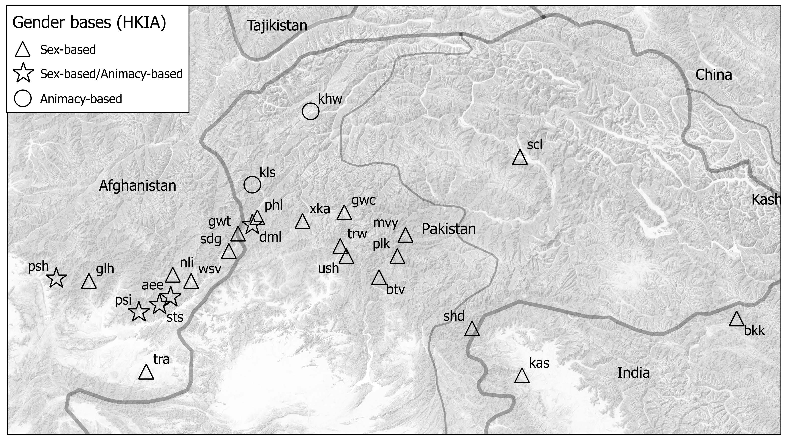
\includegraphics[width=\textwidth]{figures/10/map2_2}
\caption{Gender bases in HKIA languages}
\label{fig:Lilje:2}
\end{figure}

Second, gender is generally deeply entrenched in those languages that have a sex-based system. Especially in \ili{Kashmiri} and \ili{Shina}, i.e.\ the languages mainly spoken in the eastern part of the region, gender agreement is displayed with a wide range of targets. In a number of those languages, it is intertwined with person agreement in their verbal morphology, and we also noted some examples of gender agreement being extended to further targets. \ili{Kashmiri} and some of the \ili{Shina} languages have gender agreement with demonstratives, and it is only in these languages that we also find sex-based pronominal gender. Gender in some of the \ili{Kohistani} languages, spoken in the central part of the region, is almost equally pervasive. However, the lack (or loss) of direct object agreement in a few of those languages and the subsequently lower frequency of gender agreement with noun phrases low in the animacy hierarchy may in the long run weaken the masculine--feminine differentiation in parts of the vocabulary where sex plays no role in assignment. Accusative verbal alignment, along with relatively few agreement targets, is probably in some ways related to the erosion of sex-based gender in the Kunar languages in the western part of the region.

In \ili{Kashmiri}, \ili{Kohistani} and \ili{Kunar}, possessive modifiers are frequently targets of gender agreement. \ili{Pashai}, at the western extreme, shows a diverse picture when it comes to gender pervasiveness. As mentioned before, gender may be lost altogether in some varieties at the western periphery of Pashai; whereas in e.g.\ SE \ili{Pashai}, where direct object agreement in parts of the paradigm co-occurs with subject agreement in transitive clauses, such distinctions are frequently displayed also for inanimates. The grammatical pervasiveness of animacy-based gender is nowhere near the pervasiveness of sex-based gender, and its targets are almost invariably restricted to copula verbs and auxiliaries. The (split-)ergative pattern with object agreement in SE \ili{Pashai} is possibly a factor that may point to a higher frequency of actual and potential contrasts in animacy being expressed than in the solidly accusative languages \ili{Khowar} and \ili{Kalasha}.

Third, when it comes  to assignment criteria, the usual pattern for the sex-based systems is one of straightforward semantic assignment for humans and higher animates, and a combination of various factors (semantic, morphological and phonological) involved in the assignment of gender for lower animates and inanimates. In the animacy-based systems or sub-systems, geographically almost exclusively found at the western end of the region, semantics is the sole criterion. It also seems likely that a shift from largely non-semantic gender, such as the one in most of the \ili{Indo-Aryan} languages, to largely semantic gender, is taking place in \ili{Dameli} (and possibly also in \ili{Shumashti}).

As already noted, speakers of \ili{Hindu Kush Indo-Aryan} languages are and have been in contact with speakers of a number of other languages spoken in the region. Let us therefore take a look at these other languages and genera, in order to relate the above findings to areality beyond \ili{Indo-Aryan}.

\textbf{Other \ili{Indo-Aryan} languages.} In all four of the region's non-\ili{Hindu Kush Indo-Aryan} languages (\ili{Hindko}, \ili{Pahari-Pothwari}, \ili{Gojri} and \ili{Domaaki}), we find a sex-based two-term system typical of \ili{Indo-Aryan} (\citealt{Rehman2011}; \citealt{Weinreich2011}; \citealt{Kogan2011}; \citealt[105--201]{Losey2002}). Apart from the obvious semantic assignment of humans and other higher animates according to biological sex, lower animates and inanimates are found in the masculine and feminine classes alike. Like in many of the HKIA languages,\il{Hindu Kush Indo-Aryan} at a minimum, a sub-set of nouns have overt phonological markers; and at least in \ili{Gojri} and \ili{Domaaki}, there is a certain co-variation between gender and declensional class membership. All four languages display gender agreement with adjectives and verbs, and in addition adnominal demonstratives agree in gender in \ili{Gojri} and \ili{Domaaki}, and possessives in \ili{Gojri}. Only \ili{Gojri} shows evidence of pronominal differentiation. There are no targets of any non-sex-based agreement in any of these languages, and no observed pronominal differentiation related to animacy.

These languages are (apart from the small \ili{Domaaki} enclave in the far North) mainly spoken in the southeastern part of the region, and conform in all major aspects to the pervasive sex-based gender patterns found in the HKIA languages\il{Hindu Kush Indo-Aryan} in the same part of the region, i.e.\ \ili{Kashmiri} and various \ili{Shina} and \ili{Kohistani} varieties. It is fair to assume a high level of prolonged language contact between at least \ili{Kashmiri} and one or more of the languages of the \ili{Punjabi} continuum, whether known as Pahari, Pothwari or \ili{Hindko}, and possibly also between some of the eastern \ili{Kohistani} languages and \ili{Hindko}. However, in most of the areas where there is some overlap between speakers of HKIA and speakers of other \ili{Indo-Aryan} languages, there is no clear dominance relationship, perhaps with \ili{Hindko}-dominated parts of Pakistan-held Kashmir as an exception \citep[219]{Rehman2011a}. Both \ili{Gojri} and \ili{Domaaki} are examples of low-status languages vis-à-vis almost any other language communities that they have been in contact with (\citealt[2--4]{Losey2002}; \citealt{Weinreich1999}), and in spite of some intra-regional variations related to the relative socioeconomic status of the Gujar community (\citealt[98--99, 143--144]{Hallberg1992}), there is no evidence of any significant influence exerted by \ili{Gojri} on any of the HKIA languages.\il{Hindu Kush Indo-Aryan}

\textbf{\ili{Iranian} languages.} \ili{Iranian} languages are predominantly found in the western half of the outlined region. They belong to different groupings, and their presence, and relative influence, in the area are of very different time depths. Of the nine \ili{Iranian} languages represented, only three \textendash{} \ili{Pashto}, \ili{Shughni} and \ili{Munji}/Yid\-gha \textendash{} display a sex-based gender system of some kind (\citealt{Bashir2009}; \citealt{Edelman2009b,Edelman2009a}; \citealt{Kieffer2003,Kieffer2009}; \citealt[110--167]{Morgenstierne1938}; \citealt{Robson2009}; \citealt{Skjaervo1989}; \citealt{Windfuhr2009}). In \ili{Munji}/\ili{Yidgha}, gender as a whole is probably in radical decline. In \ili{Shughni}, the gender categories show evidence of having restructured as to form a system of semantic classes rather than primarily being assigned on the basis of sex. Only in \ili{Pashto}, which is also the language in the closest long-time contact with \ili{Indo-Aryan}, do we find a two-term system akin to the typical \ili{Indo-Aryan} one, with adjectives, verbs and adnominal demonstratives as agreement targets, and a certain co-variation between gender and declensional membership. \ili{Pashto} and \ili{Shughni} are the only \ili{Iranian} languages in the sample that express pronominal gender. The rest of the \ili{Iranian} languages of the region have long since lost the sex-based gender systems (masculine--feminine--neuter and masculine--feminine) that characterised their proto-languages (\citealt[71]{Skjaervo2009a}; \citealt[204]{Skjaervo2009b}; \citealt[288]{Yoshida2009}; \citealt[242--243]{Durkin-Meisterernest2009}). Although animacy distinctions are not part of agreement morphology, animacy does play a role in various forms of \ili{Persian}, as certain plural allomorphs are found almost exclusively with animate nouns (\citealt[431]{Windfuhr2009}), and animacy or humanness, along with register, also governs pronominal choices (\citeyear[435]{Windfuhr2009}).

It is notable that it is exactly in the transitional area between \ili{Iranian} and \ili{Indo-Aryan}, i.e.\ in the western-most part of the region, that we find both a number of \ili{Iranian} languages without gender, and those HKIA languages\il{Hindu Kush Indo-Aryan} and dialects that have either lost sex-based gender altogether, or are in the process of shifting away from a primarily sex-based system to a system where animacy distinctions are becoming grammaticalized alongside an existing sex-based system. The gender-reduced systems are found primarily in the northwest, and the systems with overlapping sex-based gender and animacy in the southwest. There is possibly a correlation between gender-preserving \ili{Pashto} being the most influential language of wider communication in the southwest and the retention of a masculine--feminine contrast in e.g.\ most \ili{Pashai} and \ili{Kunar} varieties. This is in contrast with the \ili{Chitral} languages, which show evidence, in many parts of their language systems, of long-standing and far-reaching contact with gender-reduced \ili{Iranian} languages in particular, and with a larger Central Asian contact zone in a more general sense (\citealt[176--177]{Bashir1996}). Of particular interest is the now historical but crucial contact between speakers of HKIA \ili{Khowar} and \ili{Iranian} \ili{Wakhi}. While \ili{Wakhi} of today is the less influential of the two in areas where they overlap, the relationship was most likely of a symmetrical kind in a remote past, as evidenced in cross-borrowing of basic vocabulary (\citealt{Morgenstierne1936}; \citealt[441--442]{Morgenstierne1938}; \citealt[208--210]{Bashir2007}). Different varieties of gender-less \ili{Persian}, whether literary \ili{Persian}, \ili{Dari} or \ili{Tajik}, have also had a significant (and recent) impact on the languages of \ili{Chitral} and adjacent areas across the Afghanistan border in the northwestern corner of the Hindu Kush region, as a learned language and a lingua franca.

\textbf{\ili{Nuristani} languages.} In three of the five \ili{Nuristani} languages we find a two-term system of the \ili{Indo-Aryan} type: in \ili{Waigali} (\citealt[39--91]{Degener1998}), \ili{Ashkun} (\citealt{Morgenstierne1929}; \citealt{Morgenstierne1934b}; \citealt{Morgenstierne1952}; \citealt{Buddruss2006}; \citealt{Grjunberg1999}) and \ili{Kati}/\ili{Kamviri} (\citealt{Strand2015}; \citealt[59--71]{Edelman1983}), whereas its presence in \ili{Prasun} is doubtful (\citealt{Morgenstierne1949}; \citealt[69]{Buddruss2017}). The available data for the remaining language, \ili{Tregami}, is insufficient to draw any conclusions \citep{Morgenstierne1952}. Only \ili{Kati}/\ili{Kamviri} displays pronominal gender differentiation.

Although there is evidence for Nuristan and the \ili{Nuristani} languages as an ancient centre of small-scale diffusion (\citealt{Liljegren2017a}), \ili{Nuristani} stands in most aspects, especially in more recent times, at the receiving end of contact-induced change, especially from \ili{Iranian} \ili{Pashto} and \ili{Persian} \citep[103]{Degener2002}. As far as gender is concerned, the possible erosion in \ili{Prasun} may be attributable to the same areal influences from adjacent and influential gender\hyp{}deprived \ili{Iranian} languages, as was already suggested above in regard to the HKIA \ili{Chitral} languages.

\textbf{\ili{Turkic} languages.} There is a general absence of gender distinctions in \ili{Turkic} languages, whether as overt markers of nouns or as an agreement feature \citep[530]{Kornfilt2009}. Neither are there any pronominal distinctions in these languages. This is equally true of the two \ili{Turkic} languages, \ili{Uzbek} \citep{Boeschoten1998} and \ili{Kirghiz} \citep{Kirchner1998}, spoken by populations at the northern periphery of the Hindu Kush region.

There is no present-day overlap, or at best marginally so, between any of the HKIA communities and any of the relatively nearby \ili{Turkic}-speaking groups. However, it has been suggested that at least the northern-most fringes of the Hindu Kush, together with the Pamirs and perhaps a larger region to the North, form a contact area (\citealt{Edelman1980}; \citealt[423]{Payne1989}), or alternatively a transit zone between South and Central Asia \citep[253]{Tikkanen2008}, and it is not wholly farfetched to consider \ili{Turkic} as a component of it. \citet[402--421]{Bashir1988} points out several grammatical features (e.g.\ inferentiality), primarily in \ili{Kalasha} and \ili{Khowar}, with \ili{Turkic} as their ultimate source, either mediated by certain \ili{Iranian} Pamir languages or the result of a \ili{Turkic} substrate. Besides, as \citet[104]{Johanson2013} remarks, the role of \ili{Turkic} in the massive gender loss in \ili{Iranian} at large is yet to be fully explored.

\textbf{\ili{Tibeto-Burman} languages.} Similar to what was said about \ili{Turkic}, gender in its canonical sense is not a feature generally present in \ili{Tibeto-Burman}. That is also largely true of \ili{Purik}, a \ili{Tibeto-Burman} language spoken at the southeastern periphery of the region, although there are traces of derivational morphemes indicating male or female sex (\citealt[118--127]{Zemp2013}). In closely related \ili{Balti} (\citealt[81]{Bielmeier1985}; \citealt[4]{Read1934}), the other \ili{Tibeto-Burman} language represented in the region, we find to a larger extent such markers, postposed to some nouns denoting humans or other animates, signalling the sex of the person or animal referred to: \textit{po} or \textit{pho} for male, and \textit{mo} or \textit{nɡ}\textit{o} for female (see \sectref{sec:Lilje:6} for formally and functionally similar markers in \ili{Brokskat}). This type of sex marking or gender marking on the nouns themselves, without any reflexes in agreement patterns, should not be confused with grammatical gender as we have defined it here. In the same vein, an entirely semantically transparent pronominal differentiation can be made in \ili{Balti} between human male, \textit{kho}, human female, \textit{mo}, and everything else (or when the sex is unknown), \textit{do} (\citealt[12--13]{Read1934}; \citealt[76]{Bielmeier1985}).

It is primarily the \ili{Shina} languages in the East that show traces of interaction with \ili{Tibeto-Burman} (unless we, along with \citet[305]{Tikkanen1988}, consider the possibility that some of the peculiarities of \ili{Kashmiri} vis-à-vis other \ili{Indo-Aryan} languages might be attributed to an ancient Proto-\ili{Tibetan} or \ili{Sinitic} substrate). Presently, only some groups of speakers of Gilgiti Shina\il{Shina, Gilgiti} type varieties in Baltistan and the \ili{Brokskat} community can be said to stand in any such direct and significant contact relationships, and it is only in the latter case that \ili{Tibetan} plays the role of an influential donor language. It seems likely that the relationship has been more symmetrical in the past; alternatively, we would have to assume a major \ili{Tibetan} substrate in the eastern \ili{Shina}-speaking area. That would for instance explain agent-marking (as well as some of its formal reflexes) in Gilgiti as well as in Kohistani Shina\il{Shina, Kohistani} (\citealt[162--163]{Liljegren2014}; \citealt[211]{Bailey1924}; \citealt[213--214]{Hook2004}). In the gender domain, however, \ili{Tibeto-Burman} contacts do not seem to have led to any loss or restructuring in adjacent HKIA languages,\il{Hindu Kush Indo-Aryan} although we lack substantial information on gender assignment in \ili{Tibetan} loan vocabulary in \ili{Brokskat}. The continued (and perhaps strengthened) use of overt sex-marking for higher animates in \ili{Balti}, and not in \ili{Purik}, seems to point to \ili{Shina} influences on \ili{Balti}, and not the other way around.

\textbf{\ili{Burushaski}.} In the northern part of the region, in close proximity to \ili{Indo-Aryan} \ili{Shina}, \ili{Indo-Aryan} \ili{Khowar} and \ili{Iranian} \ili{Wakhi}, the language isolate \ili{Burushaski} is spoken. \ili{Burushaski} has four genders, which makes it the language with the largest number of genders in the entire region. Although the number of differentiating values differs greatly from one part of the grammar  to another, or from one target to another (including demonstratives, numerals, verbs, possessives and to some extent adjectives), there is a maximum four-way differentiation between human masculine (\textsc{hm}), human feminine (\textsc{hf}), and two non-human categories that traditionally have been given the labels \textsc{x} and \textsc{y} (\citealt[8--9]{Willson1996}; \citealt[33--34]{Berger1998}). Somewhat simplified \textsc{hm} is human male, \textsc{hf} is human female, \textsc{x} is non-human animate, and \textsc{y} inanimate. However, in reality the relationship between the genders \textsc{x} and \textsc{y} is not quite as straightforwardly related to animacy; \textsc{x} includes not only animals but also fruit and some other count nouns, whereas \textsc{y} is the gender of abstract notions and mass nouns, but also includes e.g.\ trees and buildings (\citealt[32--33]{Yoshioka2012}). \ili{Burushaski} displays verbal agreement in gender and number with the subject as well as with the direct object of transitive clauses, as can be seen in example (\ref{ex:Lilje:17}), the first by means of a suffix and the latter by means of a prefix.

\ea
\label{ex:Lilje:17}
\ili{Burushaski} \citep[17]{Willson1996}\\
\gll hilés-e dasín-mo r toofá-muts píiš \textbf{ó}{}-t-\textbf{imi}.   \\
boy-\textsc{erg} girl-\textsc{obl.f} to gift\textsc{(x)-pl.abs} present \textsc{3pl.x}{}-do-\textsc{3sg.hm.pst}   \\
\glt `The boy presented gifts to the girl.'
\z

Gender is also pronominal, but in that case \textsc{hm} and \textsc{hf} are normally neutralised, whereas \textsc{x} and \textsc{y} both have distinct forms of pronominally used demonstratives (\citealt[81--82]{Berger1998}).

As \ili{Burushaski} represents one of the oldest, possibly the very oldest surviving, linguistic layer in the Hindu Kush region,%
\footnote{%
As pointed out to me by Johanna Nichols (p.c.), this makes perfect sense in terms of linguistic geography: a language isolated along different rivers at the highest inhabitable level is almost certainly the earlier one in and has been cut off in its former lower reaches by uphill spreads of other languages.}  it is particularly interesting from an areal point of view. While occupying a very modest territory today, the precursor of \ili{Burushaski}, or other languages perhaps (but not necessarily) closely related to \ili{Burushaski}, in all likelihood had a wider geographical scope before the advent of \ili{Indo-Iranian} languages. It has been suggested that such substratal influence underlies some features found across \ili{Iranian}, \ili{Indo-Aryan} and \ili{Burushaski} (\citealt{Tikkanen1988,Tikkanen1999}; \citealt[408--420]{Bashir1988}; \citealt{Edelman1980}). Bashir in particular attributes the gender development in the \ili{Chitral} languages to \ili{Burushaski} rather than to \ili{Iranian}, emphasizing the emergence of animacy-based contrasts. Along the same lines, \citet[423]{Payne1989}, mainly referring to Èdel'man's proposed convergence area, attributes the shift from formal-semantic to ``purely'' semantic assignment in \ili{Iranian} Pamir languages to a substratum related to or similar to \ili{Burushaski}, with special reference to a strikingly similar four-way differentiation in \ili{Iranian} Yazghulami (female human, male human, animal and inanimate), a language situated in today's Tajikistan, only marginally outside the Hindu Kush region as defined here.

\section{Conclusions}

We are now in a position to summarise and draw some overall conclusions regarding the presence and distribution (geographically and subclassification-wise) of various gender properties in \ili{Hindu Kush Indo-Aryan} (see \figref{fig:Lilje:3}).

There are two types of gender systems in the HKIA languages.\il{Hindu Kush Indo-Aryan} A fairly typical New \ili{Indo-Aryan} sex-based two-gender system is present in the majority of the HKIA languages,\il{Hindu Kush Indo-Aryan} and in five of the six subgroups. However, it is curiously missing altogether in the two \ili{Chitral} group languages, \ili{Khowar} and \ili{Kalasha}, both spoken in the northwestern corner of the region. Here, instead, a two-way animacy-based gender differentiation is in place. Furthermore, these two types of gender systems are combined in another few HKIA languages,\il{Hindu Kush Indo-Aryan} all of them found in the same part of the larger region, more or less adjacent to the \ili{Chitral} languages. In one of the latter languages, \ili{Dameli}, the inherited sex-based gender system is most likely subject to an ongoing process of erosion, and grammaticalized animacy-distinctions have emerged, although largely in complementary distribution with remaining sex-differentiation. In many of the varieties of \ili{Pashai}, the western-most extension of HKIA, an animate--inanimate differentiation serves as a sub-gender distinction within the main masculine--feminine division.

As for the entrenchment of gender, we observed important differences between the sub-groups, forming a slight decline in pervasiveness moving from East to West. However, there is also a correlation between the presence of object agreement and the reinforcement of formal gender assignment (particularly applicable to inanimate nouns), with object-agreeing languages clustering in the South, while such HKIA languages\il{Hindu Kush Indo-Aryan} are lacking altogether in the North. As for the pervasiveness of animacy-based gender, it was similarly suggested that its functional load is higher in systems with ergative verbal alignment (such as in \ili{Pashai}) than in those with a purely accusative system (such as in the \ili{Chitral} group), the latter a subject for more refined, preferably corpus-based, studies. Sex-based pronominal gender is a typical Eastern feature, exclusive to \ili{Kashmiri} and the \ili{Shina} group, whereas the evidence for animacy-based pronominal gender is scanty and does not allow for any further generalizations.

The weight that different assignment criteria have varies from language to language, and is a topic for which more detailed language-specific studies are needed. At a general level, there is a correlation between primarily sex-based gender and semantic-formal assignment criteria on the one hand; and a correlation between animacy-based gender and more straightforward semantic assignment criteria on the other. While gender in \ili{Indo-Aryan} in general often involves declensional differences \citep[219]{Masica1991}, this is not a general tendency in the HKIA languages.\il{Hindu Kush Indo-Aryan}

As far as overall complexity is concerned, a few of the HKIA languages stand out, either as being of higher than average complexity or of lower than average complexity. Languages of the first kind are primarily found in the south-westernmost part of the region; these are a handful of languages in which sex-based and animacy-based gender overlap while their targets remain largely distinct. In a single language, \ili{Kashmiri}, spoken in the south-easternmost part of the region, high complexity is instead related to a high number of target domains. The languages of the second kind are those two (\ili{Kalasha} and \ili{Khowar}) in which gender is exclusively animacy-based, and another language (\ili{Grangali}) in which agreement has been reduced to a single target domain.


\begin{figure}
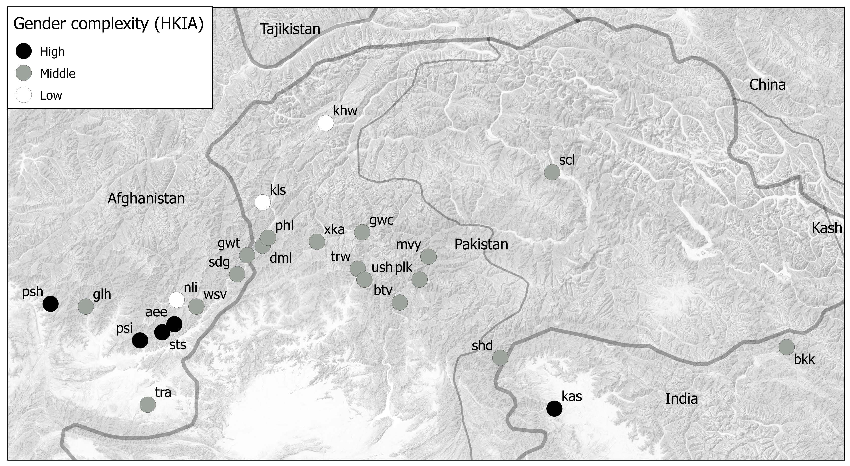
\includegraphics[width=\textwidth]{figures/10/map3_2}
\caption{Gender complexity in HKIA languages}
\label{fig:Lilje:3}
\end{figure}

The geographical distribution of gender properties within HKIA is clearly parallel to cross-genera distribution within the region. Adjacent to the main (non-HK) \ili{Indo-Aryan} continua to the Southeast as well as to \ili{Pashto}, one of the more important gender-preserving \ili{Iranian} languages, in the South, is where we find the most pervasive sex-based gender systems in HKIA. At the other end, i.e.\ the Northwest, the gender-less or gender-reduced HKIA languages\il{Hindu Kush Indo-Aryan} border with the larger \ili{Iranian}-dominated region of West and Central Asia, where sex-based gender is a rare or eroding feature, in its turn adjacent to the \ili{Turkic} belt of inner Asia where gender is altogether lacking. This patterning is clearly in line with Nichols' (\citeyear[303]{Nichols2003}) characterization of gender as a stable feature, but only as long as related languages with inherited gender are geographically clustered. We can thus expect to find that languages that have lost this feature are indeed neighbours of one another or are surrounded by non-related languages. This makes sense if we consider Morgenstierne's (\citeyear[51]{Morgenstierne1932}) hypothesis that the common ancestor of the two ``sex-less'' languages \ili{Khowar} and \ili{Kalasha} represents the earliest northward migration of Indo-Aryans into this region. For a prolonged period this language must have been a relatively minor component in an area where non-\ili{Indo-Aryan} (perhaps \ili{Burushaski}-related, or now entirely lost) languages dominated (\citealt{Tikkanen1988}; \citealt[92--94]{Parpola2002}), at the time isolated from the rest of the \ili{Indo-Aryan} varieties from which today's HKIA languages\il{Hindu Kush Indo-Aryan} derive. It is also fair to assume that groups of speakers of some of those other languages shifted to a \ili{Khowar}-\ili{Kalasha}-type language once it became a more influential element in its new environment.

Perhaps, but not necessarily, related to this is the presence of animacy-based or other semantically highly transparent gender in the North and Northwest, with \ili{Burushaski} being an obvious example. While animacy-based lexical differentiation with areal manifestation very well could be the result of borrowing, it is harder to imagine such a scenario for the copula or auxiliary agreement patterns in \ili{Shumashti} and in the \ili{Chitral} and \ili{Pashai} languages (the forms themselves also reflecting a common source); instead we have to posit either very old substratal effects, or an internal development reinforced by similar differentiations already in place in neighbouring, and at the time influential, languages. The \ili{Dameli} inanimate copula form is interesting as it bears no resemblance to the forms in the other HKIA languages\il{Hindu Kush Indo-Aryan} (cf.\ examples (\ref{ex:Lilje:2}), (\ref{ex:Lilje:3}), (\ref{ex:Lilje:12}) and (\ref{ex:Lilje:13})); instead it seems to have been recruited from inherited vocabulary \citep[138]{Morgenstierne1942}. This topic, however, deserves a great deal of more detailed research, also taking data from the Pamir region (to the North of the Hindu Kush) into account.

\section*{Acknowledgements}

I would like to thank Alla-ud-din, Bahrain, Swat, for his help with digitizing questionnaire data; Noa Lange, Stockholm, for assistance in processing and annotating audio and video recordings; and Maria Koptjevskaja Tamm and Ekaterina Melin, Stockholm, for making the contents of publications in \ili{Russian} available to me. I am also thankful for the many helpful suggestions offered by Johanna Nichols, the volume editors and four anonymous peer-reviewers.

A special thanks to a number of speakers of various HKIA languages\il{Hindu Kush Indo-Aryan} participating in four collaborative elicitation workshops organized in Islamabad and Kabul in the time period 2015 to 2017, thus contributing valuable first-hand data.

This work is part of the project \textit{Language contact and relatedness in the Hindukush region}, supported by the Swedish Research Council (421-2014-631).

\section*{Abbreviations}

\begin{tabular}{llll}
%\lsptoprule
\textsc{act} 	&	 active	&	\textsc{rem} 	&	 remote	\\
\textsc{an} 	&	 animate &	\textsc{spc} 	&	 specific\\
\textsc{cv} 	&	 converb &	\textsc{stv} 	&	 stative\\
\textsc{inan} 	&	 inanimate	&	\textsc{trz} 	&	 transitivizing suffix \\
\textsc{h}& human &	\textsc{vis} 	&	 visible	\\
\textsc{ptc} &	 participle & \textsc{x} 	&	 class x (gender in	\ili{Burushaski})	\\
\end{tabular}



\begingroup
\setlength{\emergencystretch}{8em}
\printbibliography[heading=subbibliography,notkeyword=this]
\endgroup

\end{document}
